\documentclass[submission,phys]{lib/SciPost} 

%\bibpunct{(}{)}{;}{a}{}{,} % to follow the A&A style
\usepackage{graphicx}
\usepackage{comment}
\usepackage{txfonts}
\usepackage{stfloats}
%\usepackage{algorithm}
%\usepackage{algpseudocode}
\newcommand{\spz}[1] {{\texttt{\textbf{SPZ: #1}}} }
\newcommand{\eh}[1] {{\texttt{\textbf{ EH: #1}}} }
\newcommand{\LSun}{\mbox{${L}_\odot$}}
\newcommand{\MSun}{\mbox{${M}_\odot$}}
\newcommand{\Msun}{\mbox{${M}_\odot$}}
\newcommand{\RSun}{\mbox{${R}_\odot$}}
\newcommand{\MJup}{\mbox{${M}_{\rm Jup}$}}

\def\apgt{\ {\raise-.5ex\hbox{$\buildrel>\over\sim$}}\ }
\def\aplt{\ {\raise-.5ex\hbox{$\buildrel<\over\sim$}}\ }
\def\lteq{\ {\raise-.5ex\hbox{$\buildrel<\over-$}}\ }

\newcommand{\jumbo}{\mbox{JuMBO}}
\newcommand{\jumbos}{\mbox{JuMBOs}}

%\algnewcommand{\LineComment}[1]{\State \(\triangleright\) #1}
%\def\ind#1#2{\hbox{\hskip 0.0truein\hbox to 0.2truein{#1\hfil}
%	        \hbox{\hsize 6.0truein\vtop{\ni#2}\hfil}}\vskip 1pt}

%-----------------------------------------------------------------------

\begin{document} 

\begin{center}{\Large \textbf{
      The primoridal origin of Jupiter mass Binary Objects
    }}
\end{center} 

\begin{center}
  Simon F. Portegies Zwart,\\
  Erwan Hochart
\end{center} 

\begin{center}
Leiden Observatory, Leiden University, PO Box 9513, 2300 RA, Leiden, The Netherlands\\
* spz@strw.leidenuniv.nl
\end{center}

%--------------------------------------------------------------------
\section*{Abstract} {\bf 
      The recently observed population of 540 free-floating
      jupiter-mass objects, and 42 dynamically soft pairs of
      jupiter-mass planets, among which 2 with a tertiary companion,
      in the Trapezium cluster has raised interesting questions on
      their formation and further evolution.  We test various
      scenarios for the origin and survivability of these free
      floating jupiter-mass planets and Jupiter-mass Binary Objects
      (JuMBOs) in the Trapezium cluster.  The numerical calculations
      are performed by direct N-body integration of the stars and
      planets in the Trapezium cluster starting with a wide variety of
      planets in various configurations. We discuss four main models:
      $\mathcal{SPP}$ in which selected stars have two outer orbiting
      jupiter-mass planets; $\mathcal{SPM}$ where selected stars are
      orbited by jupiter-mass planet-moon pairs; $\mathcal{ISF}$ in
      which \jumbos\, form in situ together with the stars, and
      $\mathcal{FFC}$ where we introduce a population of free floating
      single jupiter-mass objects, but no binaries.  Models
      $\mathcal{SPP}$ and $\mathcal{FFC}$ spectacularly fail to
      produce enough \jumbos. Models $\mathcal{SPM}$ can produce
      sufficient free floaters and \jumbos\, but require to start with
      unrealistically wide orbits for the planet-moon system around
      the star.  The observations are best explained with in situ
      formation (model $\mathcal{ISF}$) of \jumbos.  The observed
      populations of \jumbos\, and free floating planets in the
      Trapezium cluster are best reproduced if they formed in pairs
      and as free floaters together with the other stars in a smooth
      (Plummer) density profile with a virial radius of $\sim
      0.5$\,pc.  A fractal (with fractal dimension 1.6) stellar
      density distribution works also, but requires a very high
      initial binary fraction (close to unity) among free floating
      planet-mass objects.  This would make the primordial binary
      fraction of jumbos\, even higher than the already high observed
      fraction of $\sim 8$\,\% (42/540). The fraction of \jumbos\,
      will continue to drop with time, and the lack of jumbos\, in
      Upper Scorpius could then result of its higher age, causing more
      \jumbos\, to be ionized. We then also predict that the
      interstellar density of jupiter-mass objects (either single or
      some lucky surviving binaries) is $\sim 0.05$\,\jumbos\, per
      pc$^{-3}$ (or around 0.24 per star).  }
   
%-------------------------------------------------------------------
\section{Introduction}

Recently \cite{2023arXiv231001231P} reported on the discovery of 42
Jupiter-Mass Binary Objects (\jumbos) in the direction of the
Trapezium cluster.  Their component masses range between 0.6\,\MJup\,
and 14\,\MJup\, and have projected separations between 25\,au and
380\,au.  Two of these objects have a nearby tertiary jupiter-mass
companion.  They also observed a population of 540 single objects in
the same mass range. This discovery initiates the discussions on the
origin and surviveability of weakly bound jupiter-mass pairs in a
clustered environment.

The first single free-floating jupiter-mass objects have been found in
the direction of the Trapzium cluster more than 20 years ago
\cite{2000Sci...290..103Z,2000MNRAS.314..858L,2000AGM....17..A11M}.
Many more have been found since then, for example in the young
clustered environment of Upper Scorpio \cite{2022NatAs...6...89M}, and
through gravitational microlensing surveys in the direction of the
Galactic bulge \cite{2011Natur.473..349S}.  Their abundance may be as
high as $1.9^{+1.3}_{-0.8}$ per star \cite{2011Natur.473..349S},
although a considerable fraction of these could be in wide orbits.

The origin of these free floating planets has been actively debated
\cite{2023Ap&SS.368...17M}. Star formation, from the collapse of a
molecular cloud through gravitational instability, generally is
expected to lead to objects considerably more massive than Jupiter
\cite{1976MNRAS.176..367L,2005A&A...430.1059B}, and in disks planets
tend to form with masses. As a consequence, the large population of
jupiter-mass free-floaters is often considered to result from fully
packed planetary systems \cite{2023arXiv231015603C}, or kicked out of
their orbit by encounters with other stars in the young cluster
\cite{2019A&A...624A.120V}. Single jupiter-mass free floating objects
then originally formed in a disk around a star but became single later
in life
\cite{1996Sci...274..954R,2015MNRAS.453.2759Z,2002ApJ...565.1251H,2017MNRAS.470.4337C,
  2019MNRAS.489.2280F,2019A&A...624A.120V}.  The number of
super-jupiter mass free floating planets formed in this way is
expected to be on the order of one ($\sim 0.71$) per star
\cite{2019A&A...624A.120V}, but lower-mass free floaters orphaned this
way may be much more abundant \cite{2002ApJ...565.1251H}; The origin
of relatively massive free-floaters through dynamical phenomena is
further complicated by the tendency for lower mass planets to be more
prone to ejections
\cite{2001Icar..150..303F,2013MNRAS.433..867H,2019MNRAS.489.2280F,2020MNRAS.497.1807S}.

Explaining the observed abundance and mass-function of single
free-floating jupiter-mass objects is difficult.  In particular the
large population of objects in Upper Scorpio challenges the formation
channels. With the new discovery of a large population of of paired
free floaters complicates matters even further, and puts strong
constraints about their origin. So far, binary free-floaing
planet-mass object have been rare, and were only discovered in tight
(few au) orbits \cite{2021ApJS..253....7K}.  Known interstellar
jupiter-mass binary objects include only four objects:
\begin{itemize}
\item[$\bullet$]2MASS J11193254-1137466 AB: a $5$ to 10\,\MJup\,
  primary in a $a=3.6\pm0.9$\,au orbit \cite{2017ApJ...843L...4B}.
\item[$\bullet$]WISE 1828+2650: a 3 to 6\MJup\, primary with a
  5\,\MJup\ companion in an $\apgt 0.5$\,au orbit
  \cite{2013ApJ...764..101B}.
\item[$\bullet$] WISE J0336-014: a $8.5$ to
  $18$\,\MJup\ primary with a $5$ to $11.5$\,\MJup\, companion in a
  $0.9^{+0.05}_{-0.09}$\,au orbit \cite{2023ApJ...947L..30C}.
\item[$\bullet$]2MASS J0013-1143 discovered by \cite{2017AJ....154..112K} and
  suspected to be a binary by \cite{2019A&A...629A.145E}.
\end{itemize}

Such tight pairs could have formed as binary planets (or planet-moon
pairs) orbiting a stars, to be dislodged from their parents to become
\jumbos\, \cite{2016ApJ...819..125C}.  So long only a few were
discovered such an exotic scenario seems to pose a reasonable
explanation for their existence, but the discovery of a rich
population of $42$ wide \jumbos\, \cite{2023arXiv231001231P} requires
a more thorough study on their origin.

Adopting a dynamical origin, or at least a dynamical history, we
perform direct N-body simulations of a Trapezium-like star cluster
with primordial Jupiter-mass objects (JMO) and \jumbos. Our
simulations focus on four models that could explain the abundance,
their masses, and the orbital characteristics (actually the observed
separation distribution) of the observed jupiter-mass objects in the
cluster. In this paper, we perform a rudimentary analysis on four
scenarios capable of forming \jumbos.  Alternative to forming in situ
(scenario ${\cal ISF}$), one can naively imagine three mechanisms to
form \jumbos. \cite{2023arXiv231006016W} argued that these binaries
could be explained from hierarchical planetary systems of which the
outer two planets are stripped by a passing star in a close
encounter. The two ejected planets would lead to a population of free
floating planets, but could also explain the observed population of
\jumbos.  We call this scenario ${\cal SPP}$ (for star planet-planet).

Alternatively one could imagine \jumbos\, to result from planet-moon
pairs (or binary planets) orbiting some star that is ejected to become
a \jumbo.  We call this scenario ${\cal SPM}$, for star planet-moon.

Finally, one could imagine that a sufficiently large population of
free-floating jupiter-mass objects could lead to a population of
\jumbos\,by dynamical capture of one JMO by another.  We call this
scenario ${\cal FFC}$ (free floating capture). A similar scenario was
proposed by \cite{2010MNRAS.404.1835K} for explaining very wide
stellar pairs, but the model was also adopted to account for wide
planetary orbits \cite{2012ApJ...750...83P,2018MNRAS.473.1589G}

We start by discussing some fundamental properties of the
environmental dynamics, followed by a description of models, the
numerical simulations to characterize the parameters of the acquired
\jumbos, and the resulting occurrence rates.

%--------------------------------------------------------------------
\section{The dynamical characterization of \jumbos}

The \jumbos\, discovered by \cite{2023arXiv231001231P} were located in
the Trapezium cluster. We base our analysis on the parameters derived
for this cluster by \cite{2016MNRAS.457..313P} by numerical modeling
of disk-size distributions observed in the Trapezium cluster, and
concluded that this distribution is best reproduced for a cluster
containing $\sim 2500$ stars with a total mass of $\sim 900$\,\MSun\,
and a half-mass radius of $\sim 0.5$\,pc. The results were
inconsistent with a Plummer \cite{1911MNRAS..71..460P} distribution,
but match the observations if the initial cluster density distribution
represented a fractal dimension of 1.6.  Nevertheless, for consistency
with earlier studies, we perform our analysis for Plummer as well as
for a fractal (with fractal dimension 1.6) distributions.

Adopting a Plummer distribution of the Trapezium cluster (with $r_{\rm
  vir} = 0.5$\,pc virial radius), the cluster core radius $r_c \simeq
0.64r_{\rm vir} \sim 0.32$\,pc with a core mass of 250\,\MSun, 
resulting in a velocity dispersion of $v_{\rm disp} \equiv
GM/\sqrt{r_c^2 + r_{\rm vir}^2} \simeq 0.97$\,km/s. With a mean
stellar mass in the cluster core of 1\,\MSun\, the unit of energy
expressed in the kinematic temperature kT becomes $\sim 8 \cdot
10^{42}$\,erg.

Jumbos are found in the mass range of about 0.6\,\MJup\, to
14\,\MJup\, and have a projected separation of 25\,au\, and $\sim
380$\,au.  The averaged observed values are $d=200\pm109$\,au,
$\langle M\rangle = 4.73\pm3.48$\,\MJup, and $\langle m\rangle =
2.81\pm2.29$\,\MJup. The median and 25\,\% to 75\,\% percentiles are
$d = 193.8^{+78.2}_{-114.1}$\,au $M = 3.67^{+1.31}_{-1.57}$\,\MJup,
and $m = 2.10^{+1.05}_{-1.05}$\,\MJup.

To simplify our analysis, let us assume that the observed variation in
projected distances between the two Jupiter-mass objects corresponds
to an orbital separation, and express distances in terms of semi-major
axis (see Appendix\,\ref{Appendix:A} for motivation).  In practice,
the differences between the projected separation and the actual
semi-major axis of the orbit is small. Adopting a statistical
approach, a thermal distribution in eccentricities and a random
projection on the sky, the semi-major axis is statitically $\sim 1.2$
times the projected separation.  For the observed \jumbos\, we do not
really know if they are bound, and if so, we do not know the
underlying eccentricity distribution, but in practice this difference
between projected separation and actual semi-major axis of a bound
population is negligible compared to the 25\% to 75\% uncertainty
intervals derived with the simulations.

To first order, the binding energy of jumbos then ranges between $\sim
5\cdot 10^{37}$\,erg and $1.4\cdot 10^{41}$\,erg, or at most $\sim
0.02$\,kT. This makes them soft upon an encounter with a cluster star.

The hardest \jumbo, composed of two 14\,\MJup\, planets in a 25\,au
orbit would be hard for another encountering object of less then
$17\,M_{\rm Jupiter}$.  For an encountering 1\,\MJup\, object a 25\,au
orbit would be hard only if the two planets are about three times as
massive a Jupiter.  This entails that \jumbos\, are often soft for any
encountering free floating giant planet unless they are in tight
enough orbits or the perturber is of low mass.  On average, soft
encounters tend to soften these binaries even further
\cite{1975MNRAS.173..729H}, although an occasional soft encounter with
another planet may actually slightly harden the \jumbo.  Independent
of how tight the orbit, \jumbos\, are expected to be relatively short
lived, because they easily dissociate upon a close encounter with any
other cluster member.  Once ionized they contribute to the population
of free floating single objects.  Note that in the Trapezium cluster,
even the orbits of 2MASS J11193254-1137466AB, and WISE 1828+2650 would
be soft ($\apgt 0.025$\,kT); they could have been the hardest
survivors of an underlying population.

To further understand the dynamics of \jumbos\, in a clustered
environment, and to study the efficiency of the various formation
scenarios we perform direct $N$-body calculations of the Trapezium
star cluster with a population of jupiter-mass objects in various
initial configurations.

%--------------------------------------------------------------------
\section{Model calculations}

For each of our proposed models, ${\cal ISF}$ (in situ formation of
jumbos), ${\cal SPP}$ (\jumbos\, formed via ejections of a host stars
outer planets), ${\cal SPM}$ (as planet-moon pairs orbiting a star),
and ${\cal FFC}$ (as mutual capture of free-floaters) we perform a
series of $N$-body simulations with properties consistent with the
Trapezium cluster.

Each cluster starts with 2500 single stars taken from a broken
power-law mass-function \cite{2002Sci...295...82K} between
$0.08$\,\MSun\, and $30$\,\MSun\, distributed either in a Plummer
sphere (model Pl) or a fractal distribution with a fractal dimension
of 1.6 (model Fr). All models start in virial equilibrium.  We run
three models for each set of initial conditions, with a virial radius
of 0.25\,pc, 0.5\,pc and 1.0\,pc, called model R025, R05 and R100,
respectively.  We further assume stellar radii to follow the zero-age
main sequence, and the radius of jupiter-mass objects based on a
density consistent with Jupiter ($\sim 1.33$\,g/cc).

For each of our proposed models, we initialize a population of single
JMOs and/or \jumbos\, (binary JMOs). The single (and primaries in
planet pairs) are selected from a power-law mass function between
0.8\,\MJup\, and 14\,\MJup, which is consistent with the observed mass
function \cite{2023arXiv231001231P}. We fitted a power-law to the
primary-planet mass function, which has a slope of $\alpha_{\jumbo}
=-1.2$ (considearbly flatter than Salpter's $\alpha_{\rm Salpter} =
-2.35$).

This relatively flat mass function is not inconsistent with the mass
distribution of earlier observed free floaters The first dozen
discovered free floaters already seemd to have a rather flat mass
function \cite{2000MNRAS.314..858L}, but the large statistics
available through gravitational microlensing surveys allowd a reliable
estimate of the slope, which yields $\alpha = -1.3^{+0.3}_{-0.4}$
\cite{2011Natur.473..349S}. This mass function is somewhat steeper
than the slope derived for lower-mass free floaters ($\alpha =
-0.96^{+0.47}_{-0.27}$ \cite{2023AJ....166..108S}).

For each of the four models, we have a special set of initial
configurations. The clusters all have the same statistical
representation, being either Plummer or fractal density distributions,
virialized and with a virial radius of 0.25 ,pc, 0.5\,pc and
1.0\,pc. But the distribution of JMOs and \jumbos\, varies per model.
In figure\,\ref{Fig:models} we scetsch the various models.

\subsection{Model ${\cal SPP}$: Star hierarchically orbited by two planets}

For scenario ${\cal SPP}$, we selected the star to host such a
planetary system from the 150 stars lower in mass than 0.6\,\MSun\,
and 150 more massive stars. The mid-mass point (of 0.6\,\MSun) is
almost twice the mean stellar mass in the mass function.

We select the same planet masses as for the primordial \jumbos\,
except that we have them orbiting one of the selected stars as a
hierarchical planetary system. The distance from the first planet
$a_1$ and the second planet $a_2$ (such that $a_2>a_1$) are selected
according to various criteria.  The inner orbit $a_1$ was selected
randomly between 25\,au and $400$\,au from a flat distribution in $a$.
The outer orbit, $a_2$, we typically chose to be five times larger
than the inner planet's Hill radius.  This guarantees that the
planetary systems would be rather stable when in isolation, but they
are still rather vulnerable for external perturbations.

Both planetary orbits are rather circular with a random eccentricity
from the thermal distribution between circular and $0.02$.  The mass
of the secondary planet (could be either the inner one or the outer
one) was selected randomly from a thermal distribution between a mass
ratio of 0.2 and unity. As a consequence, we have a slight preference
for planets of comparable mass, and we do have a population of $\aplt
0.8$\,\MJup\, objects, which are not observed.  This low-mass
population contributes to $\sim 7.3$\,\% of the total.

The two planets orbit the star in a plane with a relative inclination
randomly between $-1^\circ$ and $1^\circ$. The other orbital elements
are randomly taken from their isotripic distributions.

We perform an additional series of simulations with pre-specified
orbital separations for the two planets $a_1$ and $a_2$, to follow the
model proposed in \cite{2023arXiv231006016W}. The results of these
runs are presented in figure\,\ref{Fig:fjumbos_from_PP}.

\subsection{Model ${\cal SPM}$: Star orbited by a pair of planet-mass objects}

In the ${\cal SPM}$ models we initialize planet pairs (or planet with
moons) in orbit around a star. The masses of the stars, planets and
moons are selected as in the ${\cal SPP}$ model.  The planet-moon
system orbit was selected from a flat distribution in $a$ between
$25$\,au and $200$\,au, and with a eccentricity from the thermal
distribution with a maximum of $0.02$ for the planet-moon orbit.

To warrant stability of the star-planet-moon system, we chose an
orbital separation such that the planet-moon pair stays witin 1/3th of
it's Hill radius in orbit around the star, again with an eccentricity
smaller than $0.02$ taken randomly from the thermal distribution.

The planet-moon system is randomly orientation at a distance from the
star such that the planet-moon's orbital separation is one-third of
it's Hill radius.  This guarantees a stable planet-moon pair in orbit
around the selected star, but their orbits tend to be rather wide.
two jupiter-mass objects in a circular 100\,au orbit around a
1\,\MSun\, star would lead to a circum-stellar orbit of about
3488\,au. The orbital elements for the planet-moon system around the
star is subseqenly isotropically randomized.

\subsection{Model ${\cal ISF}$: Jupiter-mass objects in weakly bound orbits}

Primordial \jumbos\, (model ${\cal ISF}$) are initialized with
semi-major axis with a flat distribution between 25\,au and $1000$\,au
(in some cases $10^4$\,au), an eccentricity from the thermal
distribution between 0 and 1, but they are to remain separated at
pericenter.  The masses are selected as in model ${\cal SPP}$.  Each
is subsequently rotated to a random orientation.  The binaries are
subsequently sprinkled in the cluster potential as single objects
using the same initial distribution function as used for the stars.

\subsection{Model ${\cal FFC}$: Jupiter-mass objects as free-floating among the stars}

For the models with free-floating jupiter-mass objects, model ${\cal
  FFC}$, we sprinkle the single planets from the primary-mass function
(see model ${\cal SPP}$) in the cluster potential as single objects
using the same initial distribution function as we used for the single
stars.  These models were run with 600\,jupiter-mass objects (rather
than 300 pairs in the other models).

We performed additional runs with $10^4$ free floaters. Some of these
runs have a different lower-limit to the mass function, but we keep
the number of objects with a mass $>0.8$\,\MJup\, at 600 (assuming that
objects of lower-mass objects are unobservable).

Each simulation is stopped at an age of 1\,Myr, after which we study
the population of free floating jupiter-mass objects and the
population of \jumbos. A few simulations were extended to 10\,Myr, to
study the long term surviveability of \jumbos.

In summary; we performed the following model calculations:\\
\begin{itemize}
\item[$\bullet$] ${\cal SPP}$: As outer orbiting planets\\
\item[$\bullet$] ${\cal SPM}$: As bound planet-moon pair orbiting a star\\
\item[$\bullet$] ${\cal ISF}$: In situ formation of jumbos\\
\item[$\bullet$] ${\cal FFC}$: Free floating single planets.\\
\end{itemize}
In figure\,\ref{Fig:models} we illustrate the four models with a
schematic diagram.

\begin{picture}(100,300)
\put(0,120){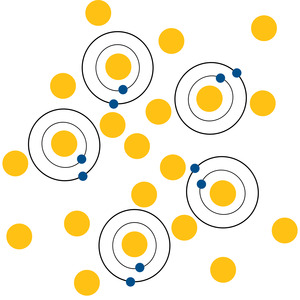
\includegraphics[width=.4\columnwidth]{figures/Model_PP.jpg}}
\put(200,120){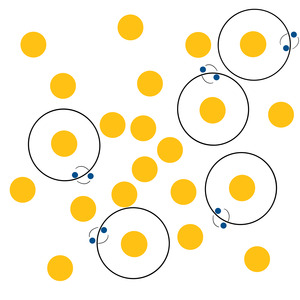
\includegraphics[width=.4\columnwidth,angle=90]{figures/Model_PM.jpg}}
\put(0,-50){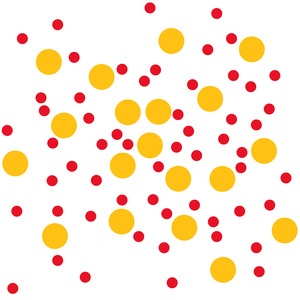
\includegraphics[width=.4\columnwidth]{figures/Model_FFC.jpg}}
\put(200,-50){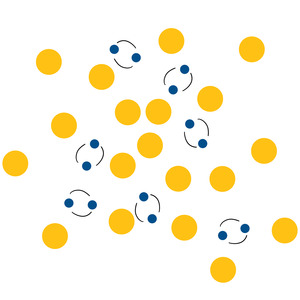
\includegraphics[width=.4\columnwidth,angle=90]{figures/Model_SF.jpg}}
\put(0,140){${\cal SPP}$}
\put(200,140){${\cal SPM}$}
\put(0,-40){${\cal FFC}$}
\put(200,-40){${\cal ISF}$}
\label{Fig:models}
\end{picture}
\vspace{2cm}

\subsection{The simulations}

All calculations are performed using 4-th order prediction-correction
direct $N$-body integrator {\sc ph4} \cite{2022A&A...659A..86P}
through the Astrophysical MUltipurpose Software Environment, or AMUSE
for short
\cite{2013CoPhC.183..456P,2013AA...557A..84P,2018araa.book.....P}.
The data files are stored in {\sc AMUSE} formatted particle sets, and
available via zenodo \url{10.5281/zenodo.10149241}, and the source
code is available at github \url{https://github.com/spzwart/JuMBOs}.

The script to run the simulations is fairly simple.  It is essentially
the same script from chapter 2 in \cite{2018araa.book.....P},
including the collision-detection stopping condition.  Runs are
performed with the default time-step parameter $\eta=0.03$, which
typically leads to a relative energy error $<10^{-8}$ per step, and
$<10^{-5}$ at the end of the run. The fractal initial condiitons with
small virial radius (0.25\,pc) are, not surprisingly, the hardest runs
to perform. The energy error in these runs can be somewhat higher at
times, but never exceed $<10^{-3}$, which according to
\cite{2041-8205-785-1-L3}, suffices for a statistically reliable
result.

Snapshots were stored every 0.1\,Myr, and the simulations were
continued until 1.1\,Myr. The data analysis is performed on the
snapshots of the 1\,Myr old cluster.

Although incorporating stellar evolution, general relativity and the
Galactic tidal field would have been straightforward, we decided to
ignore those.  We do not expect any stars to effectively lose any mass
during the short duration of the simulations, or the tidal field to
have any influence on the close encounters in the simulations.
Incorporating genera relativity would have made the calculations
expensive without much astrophysical gain.

\subsection{Finding \jumbos}

\jumbos\, are soft in terms of the average local kinetic energy of the
surrounding objects (stars and planets), and this makes them somewhat
hard to find in the numerical models.  One generally consider hard
binary paris or multiples in direct N-body simulations are finding
those soft pairs requires some extra effort.  We search for \jumbos\,
by first selecting any object in the cluster, star or planet, and find
the bound neares neighbors. Of one of these companions has another
object as nearests neighbor, we adopt that as the close pair, and the
initially selected object as the tertiary. Later, we order the
particles in terms of distance and mass, on which the eventual
designation is based. We recognice single stars $s$, and planets $p$
(although we are uncertain weather or not to call these objects
planets). Pairs of objects are then placed in parenthesis, for binary
stars we write $(s,s)$, a planetary system can be $(s,p)$ (single
planet) or $((s,p),p)$ (planet pair as in the ${\cal SPP}$ model) or
$(s,(p,p))$ (planet pair orbiting a star as in the ${\cal SPM}$
model). \jumbos\, in this terminology are indicated as $(p,p)$.

\section{Results}

The main results of the calculations are presented in the tables
table\,\ref{Tab:model_numbers} and
table\,\ref{Tab:orbital_distributions}.

In table\,\ref{Tab:model_numbers} we list per model the different
model outcomes.  The various simulations results are named after their
model designation followed by either the letter ``Pl'' for the Plummer
model, or ``Fr'' for the Fractal model.  The model name ends with the
virial radius ``R'' in parsec, here 025 indicates 0.25\,pc, 050 for
0.5\,pc and 100 for 1\,pc virial radius.

\begin{table}
  \caption{The average number of systems per simulations model
    categorized in groups.  The possible outcomes are the number of
    single stars ($n_{s}$), binaries ($n_{(s,s)}$), star orbited by a
    single planet ($n_{(s,p)}$), star orbted by two planets
    ($n_{((s,p),p))}$), single isolated planets ($n_{p}$) and \jumbos
    ($n_{(p,p)}$).  Note that we only list those objects with a mass
    $>0.8$\,\MJup.  As a consequence, the total number of planary mass
    objects does not always add up to 600.  The number of stars also
    does not always adds up to 2500 because of collisions and
    hierarchies not listed in the table.}
 \label{Tab:model_numbers}
 \centering 
 \begin{tabular}{lrrrrrrrrrrrr}
   \hline\hline
   model & $n_{s}$ & $n_{(s,s)}$ & $n_{(s,p)}$ & $n_{((s,p),p))}$ & $n_{p}$ & $n_{(p,p)}$ \\
        \hline \vspace{-0.75em}\\
${\cal SPP}$\_Pl\_R025 &  2287 &  0 & 84 & 129 & 258 & 0 \\
${\cal SPP}$\_Pl\_R050 &  2224 &  1 & 42 & 232 &  93 & 0 \\
${\cal SPP}$\_Pl\_R100 &  2204 &  0 & 19 & 277 &  26 & 0 \\
${\cal SPP}$\_Fr\_R025 &  2308 & 72 &  8 &   0 & 591 & 0 \\  
${\cal SPP}$\_Fr\_R050 &  2279 & 83 & 28 &   6 & 560 & 0 \\ 
${\cal SPP}$\_Fr\_R100 &  2327 & 64 & 27 &  10 & 553 & 0 \\

 \hline
  \hline \vspace{-0.75em}\\
${\cal SPM}$\_Pl\_R025 &  2480 & 0 & 17 & 3 & 413 & 18 \\
${\cal SPM}$\_Pl\_R050 &  2457 & 0 & 36 & 7 & 341 & 44 \\
${\cal SPM}$\_Pl\_R100 &  2464 & 0 & 22 & 14 & 394 & 15 \\
${\cal SPM}$\_Fr\_R025 &  2320 & 76 & 1 & 0 & 448 & 5 \\ 
${\cal SPM}$\_Fr\_R050 &  2293 & 90 & 2 & 0 & 444 & 17 \\
${\cal SPM}$\_Fr\_R100 &  2361 & 61 & 3 & 0 & 447 & 26 \\
  \hline
  \hline \vspace{-0.75em}\\
${\cal ISF}$\_Pl\_R025 &  2498 & 0 & 0 & 0 & 425 & 23 \\
${\cal ISF}$\_Pl\_R050 &  2498 & 1 & 0 & 0 & 362 & 48 \\
${\cal ISF}$\_Pl\_R100 &  2500 & 0 & 0 & 0 & 246 & 108 \\
${\cal ISF}$\_Fr\_R025 &  2310 & 65 & 7 & 0 & 392 & 0 \\
${\cal ISF}$\_Fr\_R050 &  2309 & 81 & 7 & 0 & 450 & 4 \\
${\cal ISF}$\_Fr\_R100 &  2345 & 73 & 0 & 1 & 454 & 6 \\
  \hline
  \hline \vspace{-0.75em}\\
${\cal FFC}$\_Pl\_R025 &  2271 & 87 & 11 & 0 & 580 & 0 \\
${\cal FFC}$\_Pl\_R050 &  2313 & 83 & 3 & 0 & 595 & 0 \\
${\cal FFC}$\_Pl\_R100 &  2331 & 75 & 5 & 0 & 593 & 0 \\
${\cal FFC}$\_Fr\_R025 &  2280 & 93 & 11 & 0 & 584 & 0 \\
${\cal FFC}$\_Fr\_R050 &  2308 & 75 & 12 & 0 & 1291 & 0 \\
${\cal FFC}$\_Fr\_R100 &  2314 & 83 & 3 & 0 & 805 & 1 \\
  \hline
 \end{tabular}
\end{table}

The ${\cal SPP}$ and ${\cal FFC}$ models systematically fail to
reproduce the observed population of \jumbos\, by a factor of 50 to
400. Changing the initial distribution in semi-major axis of the inner
orbit from a uniform distribution to a logarithmic distribution
reduces the formation rate of \jumbos\, even further.  There are some
systematic trends in terms of cluster density and Plummer versus
fractal distribution, but it is not clear how these models can lead to
\jumbos. Both models produce a considearble population of binary stars
and single planetary systems, in particular in the fractal
distributions, where the typical fraction of dynamically formed binary
stars is around 4\,\%, and the fraction of plantary sytems 0.7\,\% per
star.

Interestingly, the model that already start with some paired
configuration with a star tend to produce more binaries and planetary
systems, that the models where planet-mass objects do not orbit stars.

The high abunance of hierarchical multiple planets ($((s,p),p)$) in
the ${\cal SPP}$\_Pl and ${\cal SPM}$\_Pl models reflects some of the
initial conditions. These models also end to produce a relatively rich
population of single planet systems $(s,p)$.

The only models that produce a considerably population of \jumbos\,
are the ${\cal SPM}$ models and the ${\cal ISF}$. Where for the latter
the Plummer distributions tend to produce sufficient number of
\jumbos\, whereas the fractal model produce too few.

To further mediate the discussion, we calculate orbital parameters for
the surviving \jumbos\, in the various models.

\begin{table*}
  \caption{Simulation results for the models that produce a
    sufficiently large population of \jumbos\, to be considered
    feasable (mainly models ${\cal SPM}$ and ${\cal ISF}$). We present
    the mean values and the quartile intervales for 25\,\% and 75\,\%.
  }
\label{Tab:orbital_distributions}
 \centering 
 \begin{tabular}{llllll}
 \hline\hline
model&$\langle M \rangle$/\MJup & $\langle m \rangle$/\MJup & $\langle a \rangle$/au & $\langle e \rangle$ \\
 \hline \vspace{-0.75em} \\ 
 ${\cal SPM}$\_Pl\_R025 & $3.62^{+1.36}_{-2.68}$ & $1.12^{+0.24}_{-2.14}$ & $99.08^{+37.24}_{-36.38}$ & $0.47^{+0.18}_{-0.13}$ \\
 ${\cal SPM}$\_Pl\_R050 & $4.02^{+2.10}_{-3.71}$ & $1.74^{+0.73}_{-0.93}$ & $94.28^{+32.78}_{-78.90}$ & $0.33^{+0.19}_{-0.27}$ \\  
 ${\cal SPM}$\_Pl\_R100 & $6.93^{+4.38}_{-3.07}$ & $1.29^{+0.23}_{-1.22}$ & $140.96^{+37.10}_{-11.20}$ & $0.12^{+0.05}_{-0.27}$ \\
 ${\cal SPM}$\_Fr\_R025 & $2.66^{+1.78}_{-3.20}$ & $1.87^{+1.05}_{-0.37}$ & $35.56^{+20.57}_{-62.84}$ & $0.80^{+0.10}_{-0.18}$ \\ 
 ${\cal SPM}$\_Fr\_R050 & $9.64^{+7.02}_{-1.99}$ & $2.00^{+0.69}_{-0.58}$ & $82.76^{+21.74}_{-83.04}$ & $0.56^{+0.29}_{-0.18}$ \\ 
 ${\cal SPM}$\_Fr\_R100 & $4.60^{+2.57}_{-2.44}$ & $1.80^{+0.64}_{-2.47}$ & $73.20^{+27.21}_{-100.43}$ & $0.38^{+0.21}_{-0.13}$ \\
 \hline \vspace{-0.75em} \\ 
 ${\cal ISF}$\_Pr\_R025 & $8.12^{+3.44}_{-4.51}$ & $2.10^{+0.98}_{-1.66}$ & $112.06^{+40.76}_{-181.76}$ & $0.43^{+0.08}_{-0.19}$ \\
 ${\cal ISF}$\_Pl\_R050 & $7.00^{+3.28}_{-4.23}$ & $2.03^{+0.68}_{-0.99}$ & $296.40^{+168.53}_{-190.04}$ & $0.62^{+0.19}_{-0.12}$ \\
 ${\cal ISF}$\_Pl\_R100 & $5.25^{+2.37}_{-3.16}$ & $1.60^{+0.72}_{-1.40}$ & $457.63^{+265.29}_{-193.56}$ & $0.67^{+0.23}_{-0.14}$ \\
 ${\cal ISF}$\_Fr\_R025 &\\
 ${\cal ISF}$\_Fr\_R050 & $4.82^{+3.05}_{-4.42}$ & $1.38^{+0.75}_{-2.42}$ & $37.57^{+15.07}_{-42.46}$ & $0.77^{+0.06}_{-0.05}$ \\  
 ${\cal ISF}$\_Fr\_R100 &$10.15^{+3.75}_{-2.84}$ & $1.98^{+0.50}_{-2.13}$ & $97.05^{+47.34}_{-189.07}$ & $0.77^{+0.17}_{-0.16}$ \\
 \hline \vspace{-0.75em} \\ 
 ${\cal FFC}$\_Fr\_R100 &$6.57^{+0.00}_{-0.00}$ & $2.47^{+0.00}_{-0.00}$ & $846.35^{+0.00}_{-0.00}$ & $0.98^{+0.00}_{-0.00}$ \\
 \hline \vspace{-0.75em}  \\
 \end{tabular}
\end{table*}

The median, the 25\% and 75\% quartiles for the \jumbo\, ($(p,p)$)
distribution for primary mass, secondary mass, semi-major axis and
eccentricity are presented in table\,\ref{Tab:orbital_distributions}.
The models that preduce too few \jumbos\, to calculate the median and
quartiles are omitted.

The primary masses produced in our models ${\cal SPM}$ and ${\cal
  ISF}$, tend to be a bit on the high side, but the secondary masses
are in the observed mass range.  The ${\cal SPM}$ models all tend to
lead to orbits that are too tight. Leave out the $a<25$\,au \jumbos\,
does not improve the median orbital separation.

In terms of the orbital separation (or projected distance) the best
model seems to be the ${\cal ISF}$ Plummer model with a 0.5\,pc virial
radius, but the distributions are wide, and the 1\,pc ${\cal ISF}$
fractal model could also consistent.  We tend to prefer the former,
though, because also the number of \jumbos\, is somewhat consistent
with the observations, as well as the number of free floateers.

The eccentricity distribution in the ${\cal SPM}$ Plummer models is
systematically smaller than than in the fractal models.  In these
models, the planet-moon pairs started in almost circular orbits,
whereas in the ${\cal SPM}$ they started with higher average
eccentricities.  In the fractal models, the eccentricities are more
effectively perturbed and thermaized, whereas in the plummer models
this did seem to have happened.


\subsection{stellar and planetary collisions}

In all our simulations, we never encountered a collision between two
Jupiter-mass objects, but collisions with at least one star are not
uncommon. Plummer models tend to have fewer (or no) collisions.  the
only Plummer models in which collisions among stars were common is in
model ${\cal FFC}$ with 64, 20 and 18 collisions for those models with
a viral radius of 0.25\,pc, 0.5\,pc and 1.0\,pc, respectively.  On
average, 17\% of the collisions occurs between a star and a
planet-mass objects. Interestingly enough, the fractal models from the
same series only experience 30, 17 and 14 collisions for the same
virial radii.

In general, the fractal models all tend to experience collisions, but
mostly among stars. The collision frequency drops roughly linearly
with virial radius.

In general we argue that collision in Plummer models are rare (except
in the presence of a large population of free floating planet-mass
objects), that for the fractal models 83\% of the collisions is
between two stars and the rest between one star and one planet, and
the collision frequency is inversely proportional with initial virial
radius.

\section{Discussion}

We explore the possible origin of the rich population of jupiter-mass
binary objects (\jumbos) in the direction of the Trapezium cluster.
The main problems in explaining the observations hides in the large
number of jupiter-mass objects, their large binary fraction and the
rather wide separations. Assuming that they are bound, their orbits
would be soft for any encounter in the cluster, and they are not
expected to survive for more than a few kyr.

In figure\,\ref{Fig:Fjumbo_vs_time_model_ISF_R05} we illustrate how
the fraction of jumbos\, decreases with time in models ${\cal
  ISF}$\_Fr\_R050 and ${\cal ISF}$\_Fr\_R100.  The drop in the binary
fraction among jupite-mass objects initially drop exponentially, to
slow down after about 0.1\,Myr at a survival fraction of $\sim 2$\,\%
for the 0.5\,pc virial radius and $\sim 10$\,\% for the 1\,pc virial
radius cluster. For the latter model, the fraction of \jumbos\, drops
eventually to about 4\,\%. Both fractions are lower than the observed
8\,\%. Starting with a tighter population of \jumbos\, will help
delaying their ionization, but at the cost of losing consistency with
the distribution in the separation.

   \begin{figure}
    \centering
    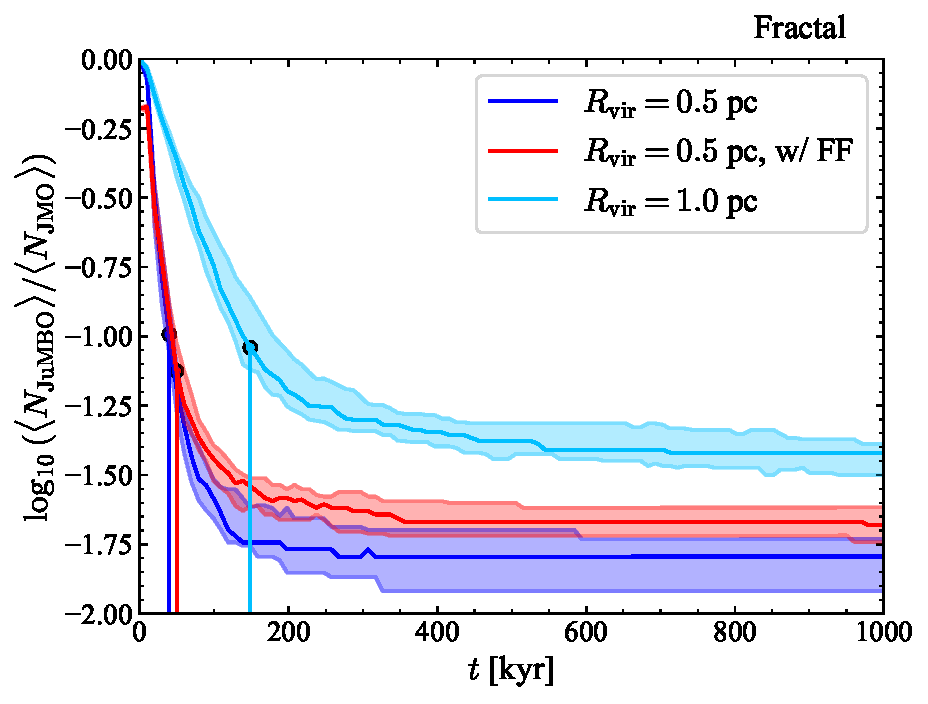
\includegraphics[width=\columnwidth]{figures/Fractal_General__fJuMBO_evol.pdf
    }
        \caption{Fraction of jumbos as a function of time for models
          ${\cal ISF}$\_Fr\_R050 and ${\cal ISF}$\_Fr\_R100. The
          former model we also calculate with a population of single
          jupiter-mass objects. The number of free floating objects is
          the same as the number if primordial \jumbos\, and their
          masses are taken from the primary mass function.}
         \label{Fig:Fjumbo_vs_time_model_ISF_R05}
   \end{figure}

An alternative explanation for the large population of pairs among the
free-floating jupiter-mass objects might be that they form late as
binaries. If, for example, they only formed in the last $\sim
0.3$\,Myr, their masses would have been understaimated, based on the
cooling curves used in \cite{2023arXiv231001231P}. with the higher
masses, the binaries would be somewhat harder, and therefore more
difficult to ionize. This would delay their destruction, and the high
binary fraction among the Jupiter-mass objects would stem from the
surviving population.

The binary fraction continues to drop, and by the time the cluster is
as old as Upper Scorpio ($\sim 10$\,Myr), very few \jumbos\, would be
left.  Although, \cite{2022NatAs...6...89M}, reported the detection of
70 to 170 jupiter-mass objects none of them would be paired.  With a
2\% fraction of \jumbos\, at an age of 10\,Myr, we would naively
expect Upper Scorpio to contain between 1 and 3 \,\jumbos, where none
were observed. Our calculations, on the other hand, did not include
primordial binaries (or higher order systems, not did we take the
effect of stellar evolution and supernovae into account. Those
processes may have a profound effect of the fraction of \jumbos,
tending to reduce them rather then increase their number.


\subsection{Failure of the ${\cal SPP}$ model}

The ${\cal SPP}$ model systematically fail to reproduce the observed
population of \jumbos\, by a factor of 50 to 400. Changing the initial
distribution in semi-major axis of the inner orbit from a uniform
distribution to a logarithmic distribution reduces the formation rate
of \jumbos\, even further.

To further explore the failure of model ${\cal SPP}$, we perform an
additional series of simulations with pre-determined inner and outer
orbital separations $a_1$ and $a_2$ using the Plummer distribution
with virial radii of 0.25\,pc, and 0.50\,pc for the stars.  According
to \cite{2023arXiv231006016W}, the eventual orbital separation of the
\jumbo\, would be consistent with the difference in orbital separation
between the two planets when orbiting the star. For this reason we
perform an additional series of runs with a mutual separation $a_2-a_1
= 100$\,au and $a_2-a_1 = 200$\,au, expecting those to lead to
consistent results in comparison with the observations, as was argued
in \cite{2023arXiv231006016W}.  The results of these simulations are
presented in figure\,\ref{Fig:fjumbos_from_PP}.

\begin{figure}
    \centering
        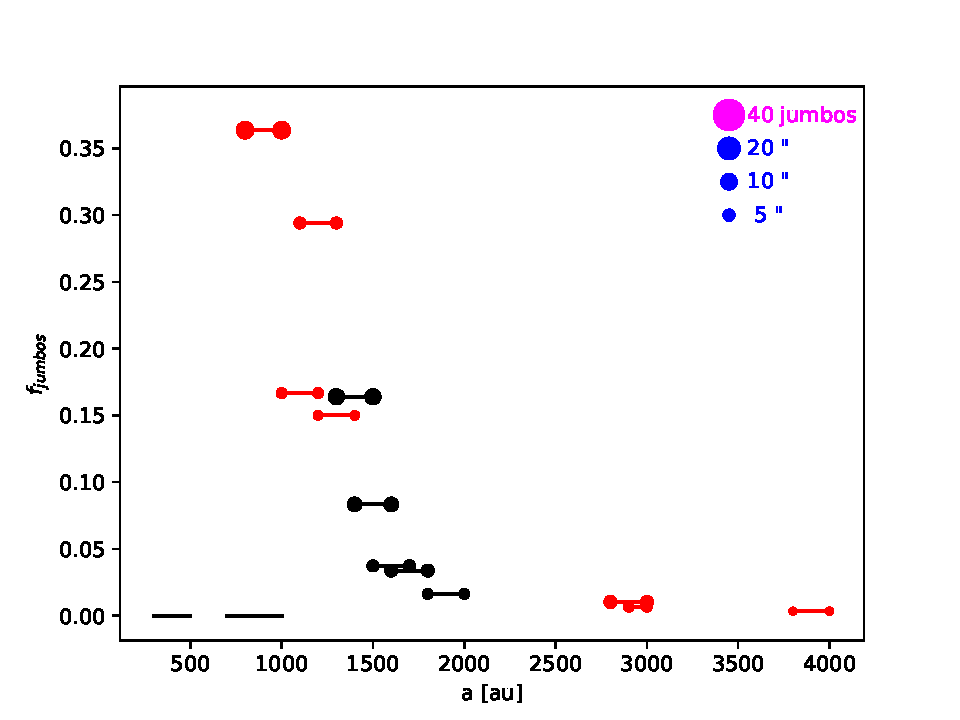
\includegraphics[width=.91\columnwidth]{figures/fig_fjumbos_from_psystems.pdf}
        \caption{The number of jumbo's produced in model ${\cal SPP}$,
          as fraction of the number of free floating planets for
          various simulations starting with a Plummer sphere with a
          virial radius of 0.5\,pc.  The bullet points along each line
          correspond with the adopted orbital separation of the two
          planets ($a_1$ and $a_2$).  The red symbols indicate an
          average orbital separations for the jumbos between 25\,au
          and 380\,au.  The black symbols are outside this regime.
          The symbol sizes give the number of jumbos (see top right
          for scaling) in the particular simulation.  }
         \label{Fig:fjumbos_from_PP}
\end{figure}

For these models the \jumbo-formation efficiency peaks for an orbital
separation $a_1 \apgt 1000$\,au, but steeply drops for smaller values
of $a_1$. As proposd by \cite{2023arXiv231006016W}, we adopt a
difference in the initial orbital distance of about $a_2-a_1 =
100$\,au or 200\,au (see figure\,\ref{Fig:fjumbos_from_PP}), which
would lead to \jumbo\, orbits in the same range.  We performed a total
of 45 calculations with various ranges of $a_1$ and $a_2$, of which 39
produced a total of 910 \jumbos. The initial mean value of $a_1-a_2 =
167\pm38$\,au, leading to a final orbital separation of the jumbos of
$a_j \sim 262\pm45$\,au.  The claim made by
\cite{2023arXiv231006016W}, that the separation distance $a_2-a_1$
leads to \jumbos\, with a similar orbital distance seems reasonable.

The rate, derived by \cite{2023arXiv231006016W}, however, appears to
be orders of magnitude smaller than they expected.  They calculate the
rate by means of 4-body scattering experiments, in which a star with
two equal-mass planets with semi-major axes $a_1$ for the inner and
$a_2$ for the other planet, encounters a single star. Their largest
cross section of roughly $a_1^2$ is obtained if the encounter velocity
$0.8v_\star/v_1$. For an encounter at the cluster's velocity
dispersion, the inner planet would then have a orbital separation of
about 900\,au around a 1\,\MSun\, star.

\subsection{The failure of model ${\cal SPP}$}

Note that an inner orbital separation of $a_1=800$\,au for a
10\,\MJup\, planet leads to a Hill radius of about 150\,au. An orbit
with $a_2=1000$\,au, is probably only marginally stable.  Still,
even in those runs the total number of \jumbos\, remains small
compared to the number of free floaters.

In \cite{2023arXiv231006016W}, the highest cross section is achieved
for the orbital velocity of the inner-most planet as fraction of the
typical encounter velocity $v1/v_{\rm disp} \sim 0.8$. With a cluster
velocity dispersion of $\sim 0.8$\,km/s, the orbital velocity roughly
1\,km/s. Around an 1\,\MSun\, star such a velocity is obtained,
assuming a Kepler orbit, at an orbital separation of 800\,au. It turns
out, that the results of the cross section calculations performed by
\cite{2023arXiv231006016W} are consistent with our direct N-body
simulation, but that the adopted initial orbital separation is too
wide in comparison with a realistically population of inner planetary
orbits for jupiter-mass planets.  Observational selection effect in
finding $\apgt 800$\,au jupiter-mass planets are quite severe, but we
consider it unrealistic to have 600 out of 2500 stars to be orbited by
such wide planetary systems. In particular, when one considers the
small sizes of the observed disks in the Trapezium cluster, which
today are all smaller than 400\,au \cite{2005A&A...441..195V}.

%%The calculation os  \cite{2023arXiv231006016W} were performed using isolated scattering e
%%\cite{2023arXiv231015603C} adopt scattering experiments to determine
%%the formation rate of jumbos from their adopted initial conditions.

\subsection{Further constraining the initial conditions for model ${\cal ISF}$}

With the current models, we can further constrain the model parameters
by repeating several calculations for better statistics and exploring
other parts of the parameter space.  We peroform this analysis for
model ${\cal ISF}$, because that model seems to be most viable for
producing a sufficiently large population of \jumbos\, and reproduces
the observed orbital characteristics.  Using the results of the
general models, we alter our initial conditions with the aim of
mimicking observations. Doing so allows us to disentangle aspects of
the cluster history, allowing for predictions on the properties of
\jumbo\, formation. These runs correspond to the middle segment of
table \ref{Tab:SF_FF_Params}.
    
For all models, we constrain $n_{\mathrm{\jumbo}} + n_{\mathrm{FF}}$ to
values reflecting the total planetary-mass population observed in
\cite{2023arXiv231001231P}, keeping in mind the survival rate of \jumbo
systems based on previous results to decide on the initial value of
$N_{\mathrm{\jumbo}}$. The range of mass ratio and mass value remains
unchanged. However, now the mass ratio follows a thermal distribution
to reflect the abundance of $q=1$ observations, whilst the mass of the
objects follows a power-law distribution with $\alpha = -1.2$. The
semi-major axis is uniformly distributed between the restricted range
$a\in[25,100]$ au. Here, the lower bound reflects the restrictions of
observational resolution in the original study
\cite{2023arXiv231001231P}.

Models Fr\_R050C and Fr0FFOC look at scenarios where the initial \jumbo\,
population has an eccentricity ranging between $e\in[0,0.2]$ sampled
from a uniform distribution. For all other models, the eccentricity
remains thermalised and ranges between $e\in[0,0.9]$.
 
\begin{table}
  \caption{Initial conditions of the various configurations. The
    nomenclature is as follows: The first letter identifies the
    cluster distribution. The number denotes the initial virial
    radius, `FF' denotes the presence of Jupiter-mass free floaters,
    `x' whether the system contains an abundance (excessive/extra)
    amount of these free floaters, `O' denotes systems whose \jumbos
    have their initial parameters constrained by the observational
    data and finally `C', systems whose initialised \jumbos\, are on
    circular orbits. Column 1: The model used. Column 2: The number of
    simulations for the given configuration. Column 3: The initial
    virial radius of the system. Column 4: The number of initialised
    \jumbos. Column 5: The number of initialised free floaters.}
        \label{Tab:SF_FF_Params}
        \centering 
        \begin{tabular}{c c c c c c}
        \hline\hline
        Model & $N_{\mathrm{runs}}$ & $R_{\mathrm{vir}}$ [pc] & $N_{\mathrm{\jumbo}}$ & $N_{\mathrm{FF}}$\\
        \hline \vspace{-0.75em}\\ 
           F05     & $20$ & $0.5$ & $500$ & $0$ \\
           F05FF   & $20$ & $0.5$ & $500$ & $500$ \\
           F1      & $20$ & $1.0$ & $500$ & $0$ \\
           P05     & $20$ & $0.5$ & $500$ & $0$ \\
           P05FF   & $20$ & $0.5$ & $500$ & $500$ \\
           P1      & $20$ & $1.0$ & $500$ & $0$ \\
           \hline
           \hline \vspace{-0.75em}\\
           F05O   & $10$ & $0.5$ & $275$ & $0$ \\
           F05FFO & $10$ & $0.5$ & $170$ & $400$ & \\
           F05OC   & $10$ & $0.5$ & $275$ & $0$ \\
           F05FFOC & $10$ & $0.5$ & $170$ & $400$ & \\
           P05FFO   & $10$ & $0.5$ & $60$  & $500$ \\
           \hline
           \hline \vspace{-0.75em}\\
           F05FFxJ & $5$ & $0.5$ & $500$ & $10^{4}$ \\
           F05FFx  & $5$ & $0.5$ & $0$   & $10^{4}$\\
         \hline                                   %inserts single line
        \end{tabular}
     \end{table}


\begin{table}
       \caption{Initial conditions of the various configurations. The nomenclature is as follows: The first letter identifies the cluster distribution. The number denotes the initial virial radius, `FF' denotes the presence of Jupiter-mass free floaters, `x' whether the system contains an abundance (excessive/extra) amount of these free floaters, `O' denotes systems whose \jumbos\, have their initial parameters constrained by the observational data and finally `C', systems whose initialised \jumbos\, are on circular orbits. Col.  1: The model used. Col.  2: The number of simulations for the given configuration. Col.  3: The initial virial radius of the system. Col.  4: The number of initialised \jumbos. Col.  5: The number of initialised free floaters.}
        \label{Tab:SF_FF_Params}
        \centering 
        \begin{tabular}{c c c c c c}
        \hline\hline
        Model & $N_{\mathrm{runs}}$ & $R_{\mathrm{vir}}$ [pc] & $N_{\mathrm{\jumbo}}$ & $N_{\mathrm{FF}}$\\
        \hline \vspace{-0.75em}\\ 
           F05     & $20$ & $0.5$ & $500$ & $0$   \\
           F05FF   & $20$ & $0.5$ & $500$ & $500$ \\
           F1      & $20$ & $1.0$ & $500$ & $0$   \\
           F05FFL  & $5$  & $0.5$ & $500$ & $500$ \\
           P05     & $20$ & $0.5$ & $500$ & $0$   \\
           P05FF   & $20$ & $0.5$ & $500$ & $500$ \\
           P1      & $20$ & $1.0$ & $500$ & $0$   \\
           \hline \vspace{-0.75em}\\
           F05O    & $10$ & $0.5$ & $270$ & $0$   \\
           F05FFO  & $10$ & $0.5$ & $200$ & $140$ \\
           F05OC   & $10$ & $0.5$ & $270$ & $0$   \\
           P05FFO  & $10$ & $0.5$ & $70$ & $400$  \\
           \hline
         \hline                                   %inserts single line
         \label{Tab:ISF_FFC_Initial}
        \end{tabular}
     \end{table}

    \subsection{$\mathcal{FFC}$: Free Floating Jupiter Mass Objects}
    In our final scenario, $\mathcal{FFC}$, we scatter $10^{4}$
    Jupiter-mass objects in the cluster with no \jumbo\, systems
    initialised. The main aim is to see the efficiency of forming
    \jumbos\, via mutual captures of free floaters. The parameters of
    the cluster and free floaters remain unchanged to those listed in
    section \ref{Sec:SF_Method}.

    \begin{table*}
         \caption{Statistics on the surviving \jumbos. $\langle ...\rangle$ gives the median, while the $\pm$ denote where the lower and upper quartile lie. Col. 1: The fraction of \jumbos\, present at the end of the simulation relative to the number initialised. Col. 2: The fraction of \jumbos\, with projected separation, $r_{\mathrm{ij}} > 25$ au. Col. 3: The mass ratio of \jumbo\, systems. Col. 4: The primary mass of the \jumbo\, system. Col. 5: The semi-major axis of the \jumbo\, system. Col. 6: The eccentricity of the system.}
        \label{Tab:SF_Res}
        \centering 
        \begin{tabular}{c c c c c c c c c}
        \hline\hline
        Model & $f_{\mathrm{surv}}$ & $f_{r_{ij} \geq 25\mathrm{ au}}$ & $\langle q\rangle$ & $\langle M_{\mathrm{prim}} \rangle\ [M_{\mathrm{Jup}}]$ & $\langle M_{\mathrm{sec}} \rangle\ [M_{\mathrm{Jup}}]$ & $r_{ij}$ [au] &$\langle a \rangle$ [au] & $\langle e \rangle$\\
        \hline \vspace{-0.75em}\\ 
           F05     & $0.02^{+0.00}_{-0.00}$ & $0.67^{+0.19}_{-0.07}$ & $0.61^{+0.21}_{-0.24}$ & $8.6^{+2.4}_{-3.3}$ & $4.2^{+3.2}_{-1.9}$ & $38^{+52}_{-18}$ & $39^{+50}_{-16}$ & $0.67^{+0.16}_{-0.19}$ \vspace{0.25em}\\
           F05FF   & $0.04^{+0.00}_{-0.01}$ & $0.61^{+0.02}_{-0.11}$ & $0.54^{+0.24}_{-0.24}$ & $8.8^{+2.7}_{-2.6}$ & $3.9^{+2.5}_{-2.0}$ & $30^{+43}_{-16}$ & $37^{+41}_{-20}$ & $0.62^{+0.14}_{-0.21}$ \vspace{0.25em}\\
           F1      & $0.04^{+0.00}_{-0.01}$ & $0.72^{+0.11}_{-0.06}$ & $0.60^{+0.20}_{-0.24}$ & $8.3^{+2.4}_{-3.0}$ & $3.8^{+2.4}_{-1.9}$ & $64^{+98}_{-40}$ & $67^{+83}_{-38}$ & $0.68^{+0.16}_{-0.19}$ \vspace{0.25em}\\
           F05FFL  & $0.03^{+0.00}_{-0.00}$ & $0.46^{+0.07}_{-0.07}$ & $0.57^{+0.31}_{-0.25}$ & $8.1^{+2.9}_{-2.7}$ & $2.7^{+3.1}_{-1.0}$ & $33^{+20}_{-18}$ & $20^{+15}_{-9}$ & $0.61^{+0.20}_{-0.19}$ \vspace{0.25em}\\
           P05     & $0.37^{+0.01}_{-0.02}$ & $0.94^{+0.02}_{-0.01}$ & $0.55^{+0.23}_{-0.23}$ & $8.3^{+2.7}_{-3.1}$ & $3.6^{+2.7}_{-1.8}$ & $233^{+234}_{-137}$ & $268^{+237}_{-152}$ & $0.68^{+0.16}_{-0.22}$ \vspace{0.25em}\\
           P05FF   & $0.52^{+0.02}_{-0.00}$ & $0.92^{+0.00}_{-0.01}$ & $0.57^{+0.21}_{-0.24}$ & $8.1^{+2.8}_{-3.2}$ & $3.4^{+2.7}_{-1.7}$ & $162^{+167}_{-94}$ & $187^{+176}_{-106}$ & $0.61^{+0.14}_{-0.18}$ \vspace{0.25em}\\
           P1      & $0.72^{+0.02}_{-0.01}$ & $0.97^{+0.00}_{-0.01}$ & $0.54^{+0.24}_{-0.23}$ & $7.8^{+3.0}_{-3.0}$ & $3.3^{+2.5}_{-1.6}$ & $344^{+271}_{-188}$ & $396^{+250}_{-206}$ & $0.68^{+0.16}_{-0.20}$ \vspace{0.25em}\\
           \hline \vspace{-0.75em}\\
           F05O    & $0.02^{+0.00}_{-0.01}$ & $1.00^{+0.00}_{-0.16}$ & $0.81^{+0.09}_{-0.17}$ & $4.0^{+2.6}_{-1.9}$ & $2.8^{+1.7}_{-1.5}$ & $61^{+46}_{-24}$ & $67^{+48}_{-22}$ & $0.67^{+0.14}_{-0.19}$ \vspace{0.25em}\\
           F05FFO  & $0.03^{+0.00}_{-0.00}$ & $0.8^{+0.02}_{-0.15}$ & $0.76^{+0.10}_{-0.17}$ & $3.4^{+3.4}_{-1.7}$ & $1.8^{+2.0}_{-0.8}$ & $44^{+37}_{-18}$ & $46^{+38}_{-22}$ & $0.69^{+0.15}_{-0.18}$ \vspace{0.25em}\\
           F05OC   & $0.02^{+0.01}_{-0.00}$ & $0.67^{+0.19}_{-0.07}$ & $0.81^{+0.10}_{-0.14}$ & $4.7^{+3.2}_{-2.7}$ & $3.6^{+2.6}_{-2.02}$ & $46^{+36}_{-26}$ & $49^{+28}_{-28}$ & $0.45^{+0.33}_{-0.23}$ \vspace{0.25em}\\
           P05FFO  & $0.76^{+0.01}_{-0.01}$ & $0.89^{+0.03}_{-0.03}$ & $0.78^{+0.12}_{-0.15}$ & $3.7^{+3.5}_{-2.1}$ & $2.1^{+2.5}_{-1.2}$ & $90^{+86}_{-44}$ & $105^{+86}_{-47}$ & $0.61^{+0.15}_{-0.17}$ \vspace{0.25em}\\
           \hline
         \hline                                   %inserts single line
         \label{Tab:Final_ISF_FFC_Results}
        \end{tabular}
     \end{table*}

   
   \begin{figure}
    \centering
        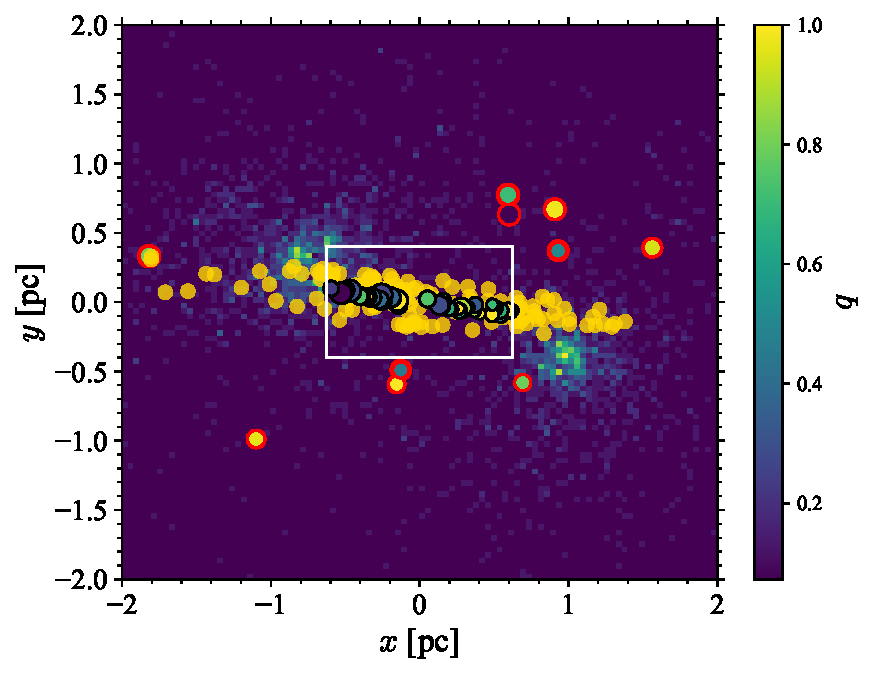
\includegraphics[width=\columnwidth]{figures/overplotting_HEATMAP.pdf}
        \caption{Schematic of a F05 simulation. The density map denotes final positions of simulated objects, the translucent yellow points observed stars taken from \cite{2016A&A...595A...1G, 2023A&A...674A...1G}. The white frame denotes the observed region in \cite{2023arXiv231001231P}, with black outlined dots denoting observed \jumbos. Red outlined dots denote the final \jumbos\, observed in our simulation.}
         \label{Fig:Overplot}
   \end{figure}

    Figure \ref{Fig:Overplot} shows the final snapshot of a F05 simulation. It represents the typical final state of simulations evolved during our $\mathcal{ISF}$ and $\mathcal{FFC}$ runs. The density map reveals the final positions of all objects simulated. Surviving \jumbos\, are scattered onto the plot with red outlines. Overlayed are also the positions of known stars (in yellow) taken from \cite{2016A&A...595A...1G, 2023A&A...674A...1G} and the positions of known \jumbos\, (black outlined points) \cite{2023arXiv231001231P}.

    Table \ref{Tab:Final_ISF_FFC_Results} summarises all our final results. We begin our discussion on the $\mathcal{ISF}$ models by looking at the general models (top segment of table \ref{Tab:ISF_FFC_Initial}). 
     
    Overall, \jumbos\, are more likely to survive in a Plummer-like cluster. Their survival rates increase by a factor of $\sim 18$ compared with likewise configurations initialised under a Fractal distribution. Even so, no configuration is successful in reproducing the $9\%$ fraction of \jumbos\, relative to free-floaters observed. Instead, in the $\mathcal{ISF}$ scenarios, the fraction of \jumbos\, to JMO free floaters ranges between $0.29\sim1.3$ for Plummer runs and $0.01\sim0.02$ for Fractals.
    
    The increase of \jumbo\, surviveability in runs including free-floaters could be due to the rare JMO-\jumbo interaction hardening the binary, also resulting in a decrease in its gravitational cross section. We believe this to be the case even though as discussed in the introduction \jumbos\, will tend to ionise, even when interacting with other JMO, since, although increasing the number of JMOs enhances the chances of two free-floaters (or a free floater and ionised JMO) settling into a newly formed binary, on average, only $0.4$ new \jumbo\, systems emerge per run for F05 runs compared to the $0.65$ in F05FF (from $1.75$ to $3.15$ between P05 and P05FF). 
    
    Figures \ref{Fig:Gen_Semi_Fractal} show the cumulative distribution function (CDF) for the semi-major axis of surviving \jumbos\, during F05, F05FF and F1 runs. The Fractal distribution efficiently prunes off any wide orbits since its violent nature provokes many encounters result in the ionisation of \jumbo\, systems, moreso the ones on wide orbits who have a larger cross-section. The tendency for \jumbos\, to ionise at any encounter is reflected by the little variation between runs of the same virial radius. We also note the tendency for \jumbos\, to ionise even when a JMO perturbs the system as reflected with the decrease in median semi-major axis between models P05 and P05FF from $\langle a\rangle\sim268$ au to $\langle a\rangle\sim187$ au.
   
   \begin{figure}
    \centering
        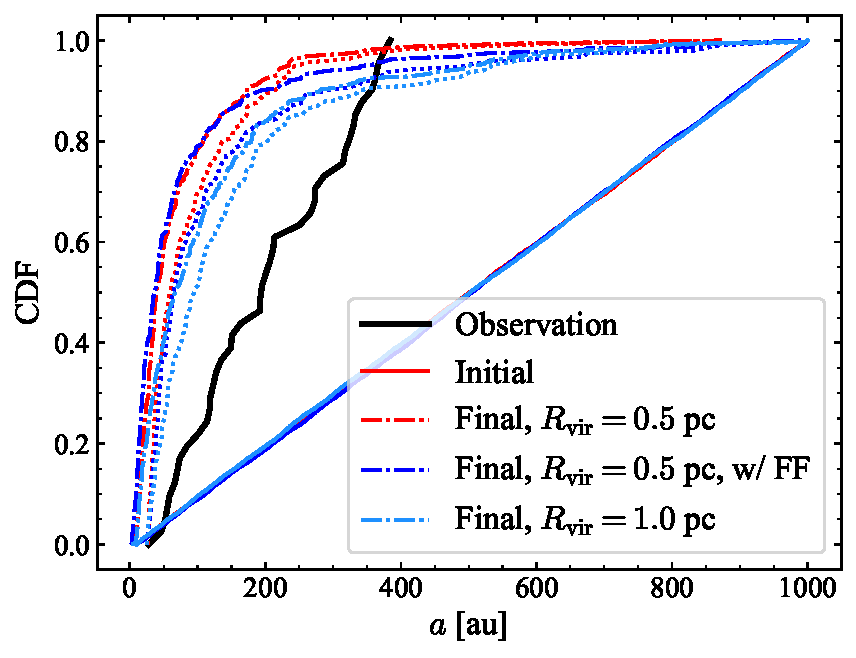
\includegraphics[width=\columnwidth]{figures/Fractal_General_sem_axis.pdf}
        \caption{CDF of surviving \jumbo\, semi-major axis distribution for models F05, F05FF, F1. Dash-dotted curves incorporate all \jumbo\, systems, whereas dotted ones only those with a projected separation exceeding $25$ au.}
         \label{Fig:Gen_Semi_Fractal}
   \end{figure}
    
    The results in semi-major axis' during the Fractal runs are much smaller than those observed, suggesting the $\mathcal{ISF}$ model fails to capture the birth of such environments. Contrariwise, and as seen in figure \ref{Fig:Gen_Semi_Plummer}, Plummer models are capable of preserving the wider orbits. This, however, is due to the environment to output similar values to those inputted since it is less violent by nature.
   
   \begin{figure}
    \centering
        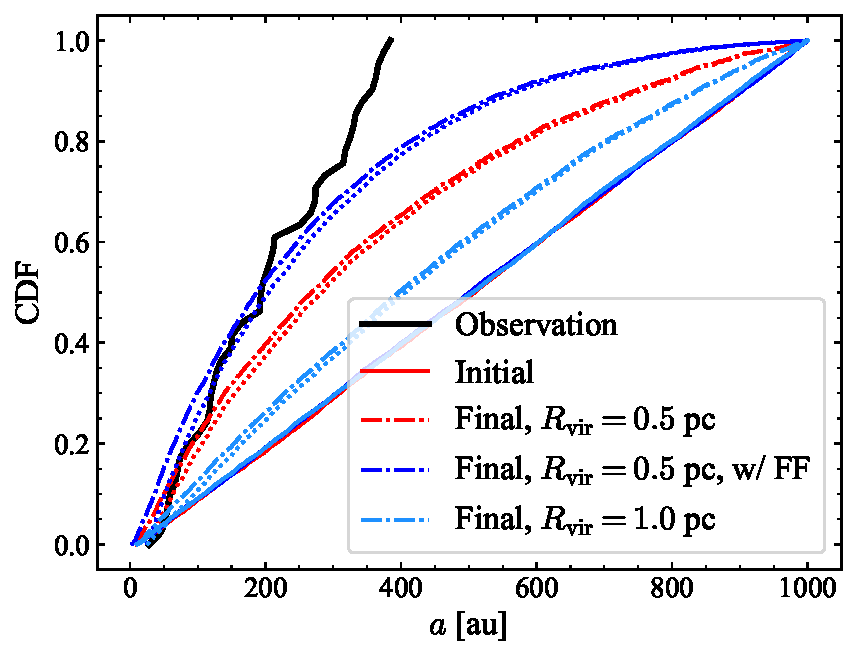
\includegraphics[width=\columnwidth]{figures/Plummer_General_sem_axis.pdf}
        \caption{CDF of surviving \jumbo\, semi-major axis distribution for models P05, P05FF, P1. Dash-dotted curves incorporate all \jumbo\, systems, whereas dotted ones only those with a projected separation exceeding $25$ au.}
         \label{Fig:Gen_Semi_Plummer}
   \end{figure}

    Indeed, keeping in mind that our \jumbos\, in these models are initialised with a uniform mass distribution, we see the uniformity reflected in the final $M_{\mathrm{prim}}$ vs. $q$ parameter space shown in figure \ref{Fig:Gen_mdistr_Plummer}. Although it also fails at reproducing observations, figure \ref{Fig:Gen_mdistr_Fractal} shows more structure and less uniformity in the distribution of \jumbos\, in ($M_{\mathrm{prim}}$, $q$)-space as reflected by the starker contrasts between contour levels and smaller high-density regions.
    
    Given this, although a correct calibration of initial conditions during Plummer runs will give back \jumbos\, with similar properties to those observed, the extent of fine tuning needed and lack of natural mechanism to remove the tail end of wide-orbit \jumbos, we can apply Occam's razor to rule it out as an initial conditions. 
    
    The omission of Plummer models is further supported since no systems formed dynamically during the runs. This contradicts with the observed presence of two triple JMO systems. Given this, we restrict ourselves to Fractal models as we believe this better represents the Trapezium cluster, a fact agreeing with \cite{2016MNRAS.457..313P}.
   
   \begin{figure}
    \centering
        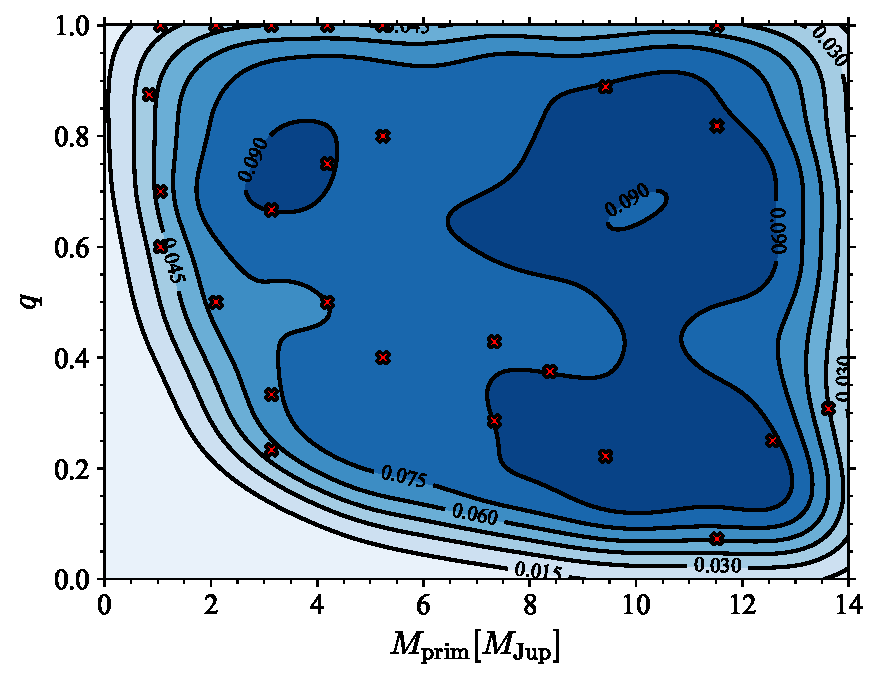
\includegraphics[width=\columnwidth]{figures/Plummer_rvir0.5_FF_mass_distr.pdf}
        \caption{Contour plot of $M_{\mathrm{prim}}$ vs. $q$ for model P05FF. Red crosses denote where observed \jumbos\, lie.}
         \label{Fig:Gen_mdistr_Plummer}
   \end{figure}
   
   \begin{figure}
    \centering
        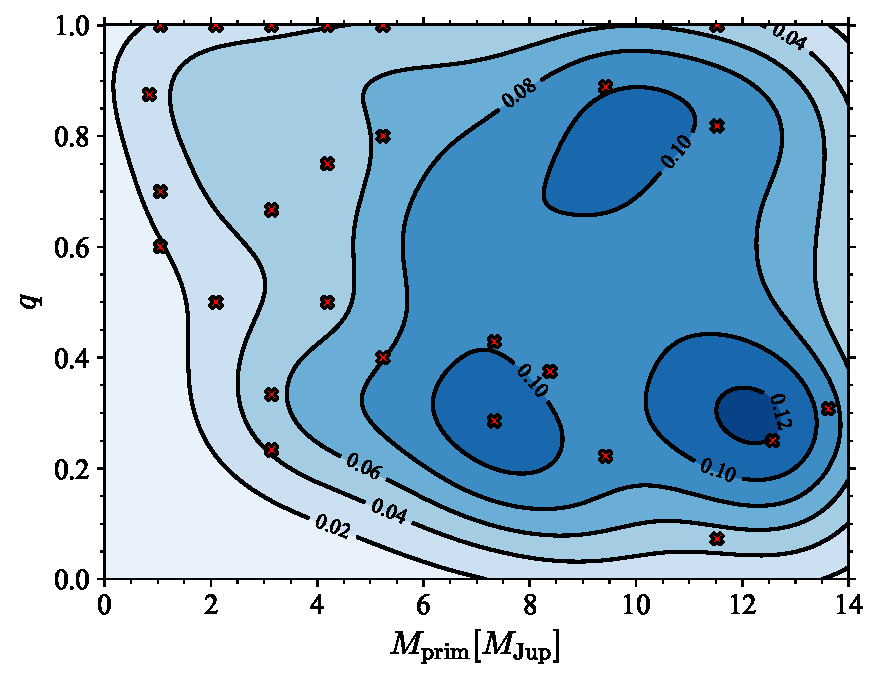
\includegraphics[width=\columnwidth]{figures/Fractal_rvir0.5_FF_mass_distr.pdf}
        \caption{Contour plot of $M_{\mathrm{prim}}$ vs. $q$ for model F05FF. Red crosses denote where observed \jumbos\, lie.}
         \label{Fig:Gen_mdistr_Fractal}
   \end{figure}

    \subsubsection{Evolving till $10$ Myr}
        Here we analyse results for a system evolved to $10$ Myr, with the aim of looking at the survival of \jumbos\, in more established systems. Overall, the \jumbo\, survival rate decreases and the ones surviving exhibit tighter orbits with $\langle a\rangle \sim 20$, a regime in which two $3\ M_{\mathrm{Jup}}$ systems become hard for $\sim M_{\mathrm{Jup}}$ interactions. 
        
        Figure \ref{Fig:Mdistr_SimTime} shows the distribution of $M_{\mathrm{prim}}$ of surviving \jumbos. The little difference  observed between F05FF and F05FFL is reflected by the similarities between their median and interquartile (IQR) range ($\langle M_{\mathrm{prim}}\rangle\sim 8.8$ and $\langle M_{\mathrm{prim}}\rangle \sim 8.1$ for F05FF and F05FFL respectively). The fact that this holds for all configurations simulated implies the ease at which \jumbo\, systems ionise upon interaction.

        Figure \ref{Fig:SimTime_MPrimQ} shows the contour plot of $M_{\mathrm{prim}}$ vs. $q$. As before, the parameter space poorly replicates the observed distribution with most of the \jumbos\, having too large a primary mass. We keep this in mind for simulations in the following subsection where we initialise \jumbos\, with a power-law of $\alpha = -1.2$, the power-law found to best fit observations.
   
   \begin{figure}
    \centering
        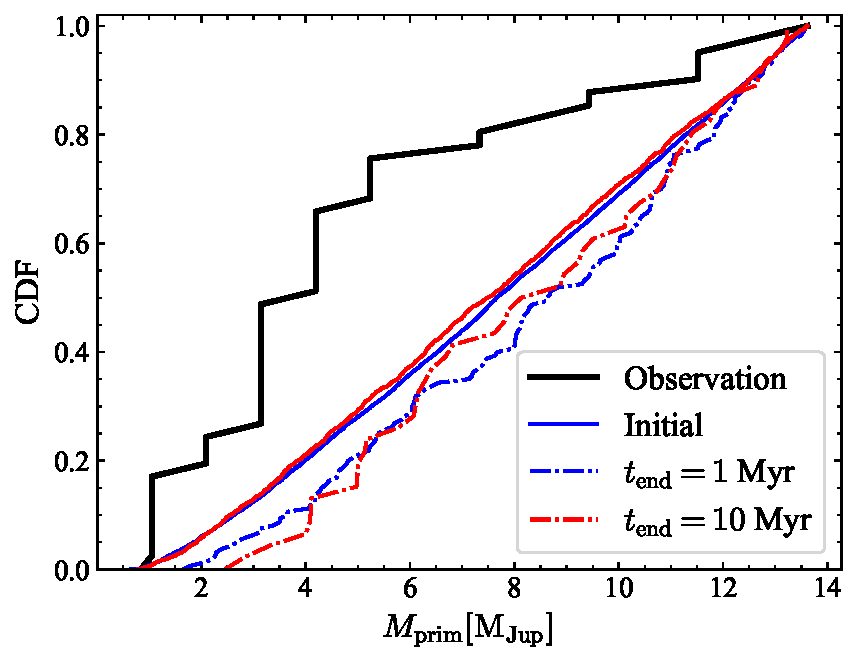
\includegraphics[width=\columnwidth]{figures/SimTime_mprim_vs_obs_.pdf}
        \caption{CDF of surviving \jumbo\, $M_{\mathrm{prim}}$ for models F05FF and F05FFL.}
         \label{Fig:Mdistr_SimTime}
   \end{figure}
   
   \begin{figure}
    \centering
        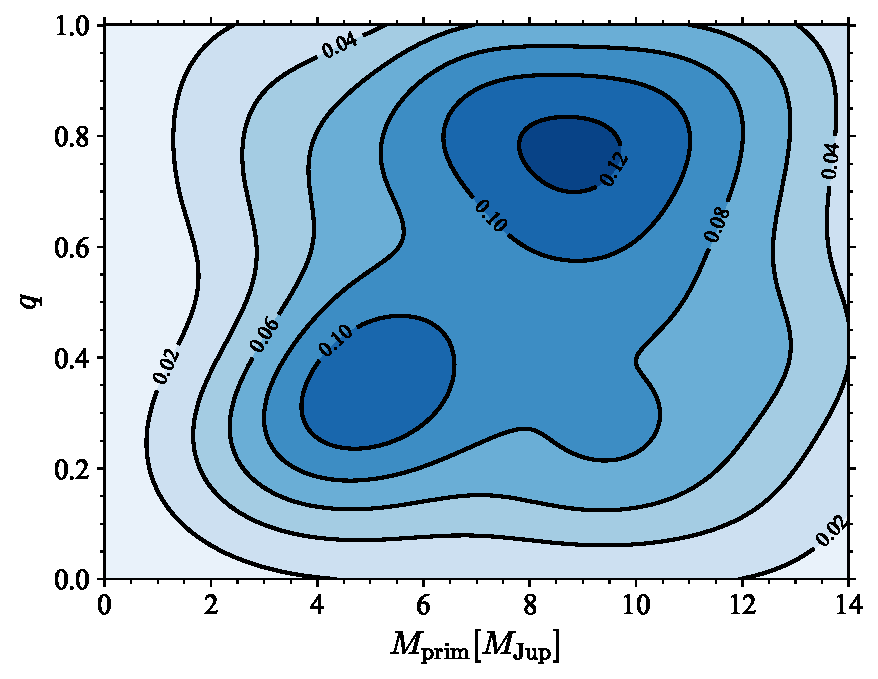
\includegraphics[width=\columnwidth]{figures/Fractal_rvir0.5_FF_10Myr_mass_distr.pdf}
        \caption{$M_{\mathrm{prim}}$ vs. $q$ contour plot for model F05FFL. Red crosses denote where observed \jumbos\, lie.}
         \label{Fig:SimTime_MPrimQ}
   \end{figure}
   
    \subsubsection{Observational Constraints}
    Our preliminary exploration allows us to rule out Plummer models and further constrain the parameter space. When applying these more restricted initial conditions, $f_{\mathrm{surv}}$ and $e$ barely changes while $a$ shows only marginal changes.

    This slight increase in $f_{r_{ij}\geq25\ \mathrm{au}}$, $\langle a\rangle$ and $\langle r_{ij}\rangle$ could be attributed to the reduction of JMO and \jumbos\, present in the environment and the smaller masses they occupy making it harder for them to destabilise wide binaries. The difference in the semi-major axis distribution between models F05, F05O and F05OC (\jumbos are initially on circular orbits) is shown in figure \ref{Fig:Semi_Fractal}. No matter the configuration, the Fractal models exhibit a natural tendency for trimming out wide binaries.
    
   \begin{figure}
    \centering
        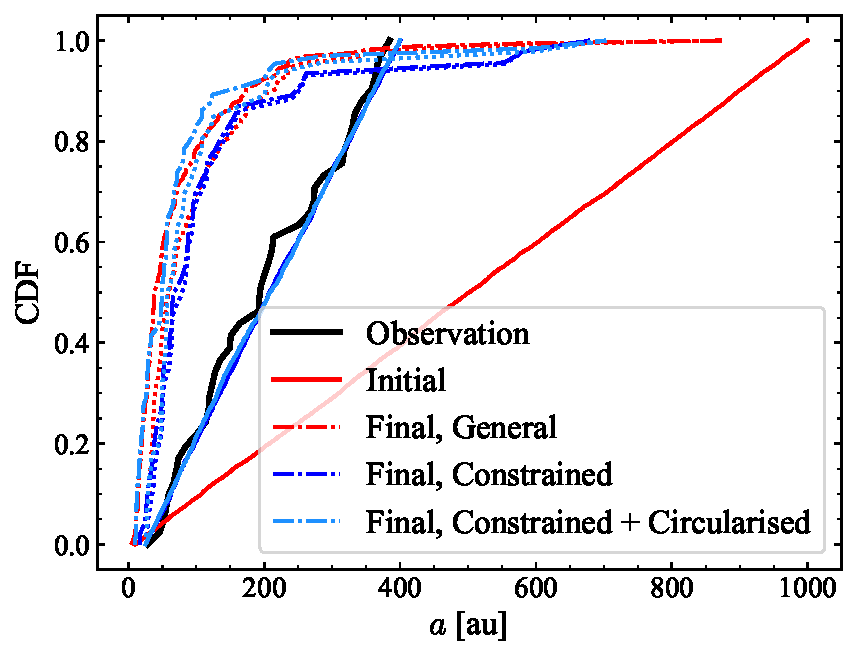
\includegraphics[width=\columnwidth]{figures/Fractal_noFF_sem_axis.pdf}
        \caption{CDF of surviving \jumbo\, semi-major axis distribution for models F05, F05O, F05OC.}
         \label{Fig:Semi_Fractal}
   \end{figure}

   Figure \ref{Fig:Fractal_mdistrCDF} shows the CDF of primary masses comparing models F05, F05O And F05OC. No matter the configuration, a similar evolution is observed where surviving \jumbos\, tend to have larger primary masses. However, unlike the F05 model, the constrained model, initialised with $\alpha = -1.25$, end up being roughly uniform in primary mass compared to the somewhat thermal appearance for F05. In doing, the median primary masses shift towards lower values while the mass ratio towards larger one. A fact reflected by the statistics shown in table \ref{Tab:Final_ISF_FFC_Results} and shown in figure \ref{Fig:FractalObs_mdistr}.
    
   \begin{figure}
    \centering
        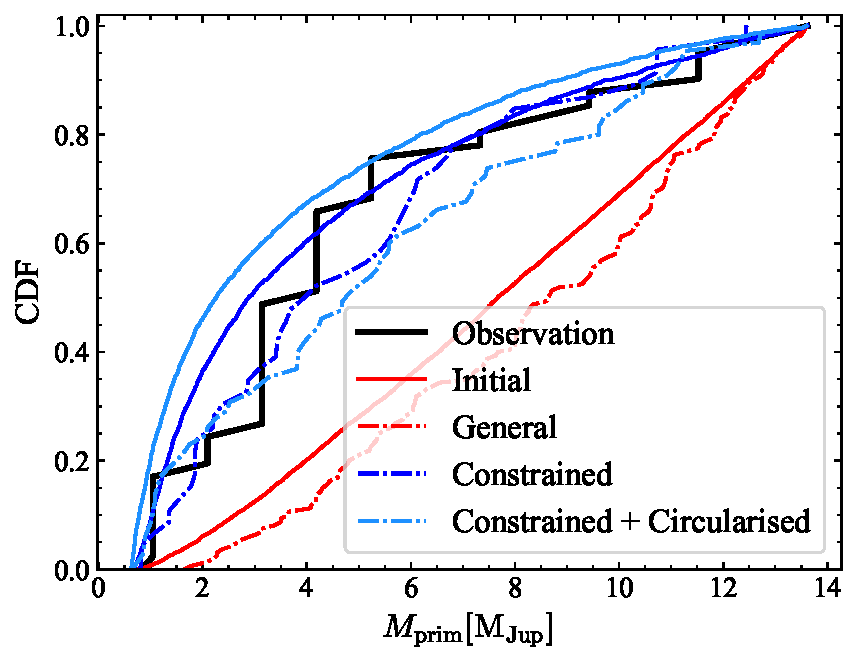
\includegraphics[width=\columnwidth]{figures/Fractal_noFF_mprim_vs_obs_.pdf}
        \caption{CDF of surviving \jumbo\, primary mass for models F05, F05O, F05OC.}
         \label{Fig:Fractal_mdistrCDF}
   \end{figure}

    Over the course of our simulation, Fractal runs exhibit a range of dynamical phenomena. The statistics of merging scenarios, and the emergence of both Jupier-mass - Stellar binary systems and $N\geq3$ systems are summarised in table \ref{Tab:Systems}.

    Jupiter-mass - stellar mergers could ................ In addition to mergers, ejection events also occured. Though no \jumbos\, were ejected, $\sim1$ JMO was ejected per simulation and $\sim 3$ stellar-mass objects.
    
    Figure \ref{Fig:MixedSys_OrbParams} shows where in $(a,e)$-space Jupiter-mass - Stellar binaries lie, with little variation between configurations. The parameter space is widely covered, with signs of low-eccentricity but very wide ($a\geq700$ au) binaries. Nevertheless, the vast majority exhibit large eccentricities and semi-major axis, reflecting their dynamical origin. The non-negligible amount of these systems emerging provide an interesting prospect of detecting ultra-cold Jupiters orbiting stars who have recently fostered them.

    Given the poor reproducability in ratios of \jumbos\, to JMO free floaters and the tight orbits of \jumbos\, we conclude that the $\mathcal{ISF}$ models are most likely not the origins of \jumbos, lending us to our final possible scenario, $\mathcal{FFC}$.

   \begin{figure}
    \centering
        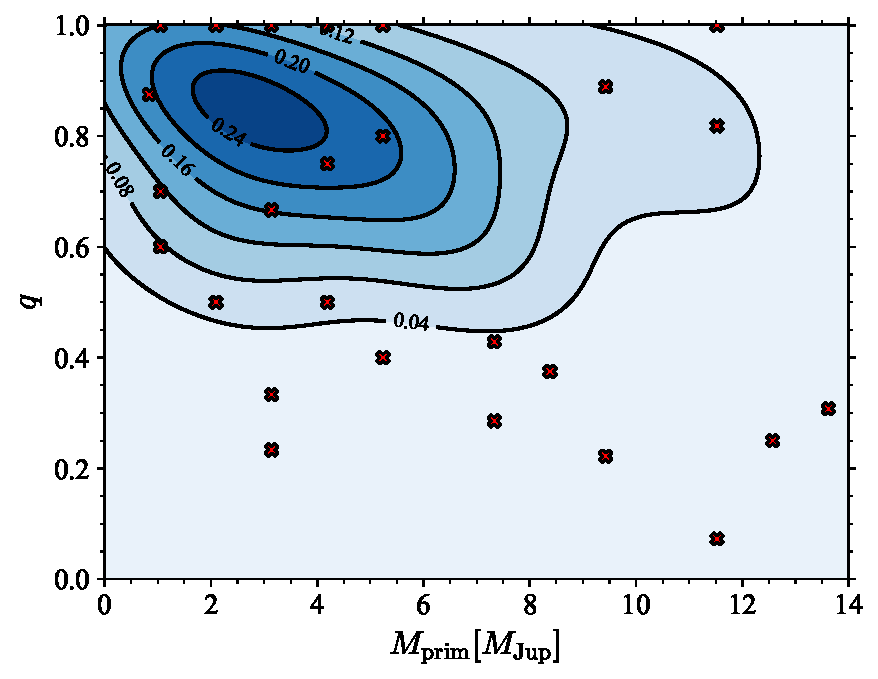
\includegraphics[width=\columnwidth]{figures/Fractal_rvir0.5_Obs_mass_distr.pdf}
        \caption{Contour plot of $M_{\mathrm{prim}}$ vs. $q$ for F05O. Red crosses denote where observed \jumbos\, lie.}
         \label{Fig:FractalObs_mdistr}
   \end{figure}
   
   \begin{figure}
    \centering
        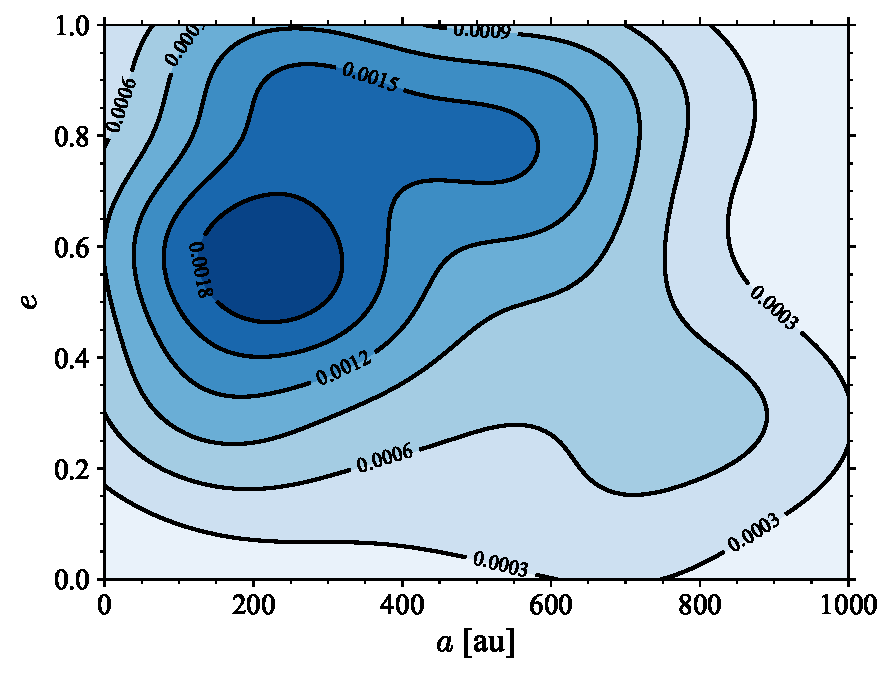
\includegraphics[width=\columnwidth]{figures/Fractal_rvir0.5_FF_Obs_sem_ecc_mixed_systs.pdf}
        \caption{$a$ vs. $e$ parameter space occupied by Star-JMO binaries during F05FFO runs.}
         \label{Fig:MixedSys_OrbParams}
   \end{figure}

    \begin{table}
         \caption{TO CHECK}
        \label{Tab:M2Events} 
        \centering 
        \begin{tabular}{c c c c c}
        \hline\hline
        Model & $\langle N_{\mathrm{JS, merge}}\rangle$ & $\langle N_{\mathrm{SS, merge}}\rangle$ & $\langle N_{\mathrm{JS}}\rangle$ &  $\langle N_{\mathrm{multi}} \rangle$ \\
        \hline \vspace{-0.75em}\\ 
           F05     & $2.5^{+0.5}_{-1.5}$ & $19^{+4}_{-7}$ & $8^{+3}_{-0}$  & $2^{+0}_{-0}$ \vspace{0.25em}\\
           F05FF   & $5.5^{+1.5}_{-1.5}$ & $21^{+2}_{-4}$ & $14^{+1}_{-3}$ & $2^{+0}_{-0}$ \vspace{0.25em}\\
           F1      & $1.0^{+1.0}_{-0.0}$ & $14^{+3}_{-5}$ & $10^{+1}_{-3}$ & $2^{+0}_{-0}$ \vspace{0.25em}\\
           F05FFL  & $5.0^{+0.0}_{-1.0}$ & $22^{+3}_{-5}$ & $1.0^{+0.0}_{-0.0}$ & $0^{+7}_{-0}$ \vspace{0.25em}\\
           \hline \vspace{-0.75em}\\
           F05O    & $2.0^{+0.8}_{-1.8}$ & $25^{+2}_{-8}$ & $4.5^{+2.8}_{-0.5}$ & $2.0^{+0}_{-0}$ \vspace{0.25em}\\
           F05FFO  & $1.0^{+1.0}_{-0.0}$ & $17^{+3}_{-1}$ & $5.0^{+1.5}_{-1.0}$ & $1.0^{+0}_{-0}$ \vspace{0.25em}\\
           F05OC   & $0.5^{+2.3}_{-0.5}$ & $20^{+5}_{-4}$ & $4.5^{+1.5}_{-1.5}$ & $3.5^{+0}_{-0}$ \vspace{0.25em}\\
           \hline
         \hline                               %inserts single line
         \label{Tab:Systems}
        \end{tabular}
     \end{table}
    \subsection{$\mathcal{FFC}$}
    

%--------------------------------------------------------------------
\section{Conclusions}

The discovery of relatively wide pairs of jupiter-mass planetary
objects in the Trapezium cluster emphasizes our limited understanding
of low-mass star and planet formation. In order to derive
characteristcs for their origin we performed simulations of
Trapezium-equivalent stellar clusters (2500 stars with a virialized
$\sim 0.5$\,pc radius) with various compositions of planetary objects
and stars.

Models in which planets form in wide circum-stellar orbits, as
proposed by \cite{2023arXiv231006016W}, produce many single free
floating planets, but an insufficient number of planet pairs per
cluster. The ratio of single to pairs of planets is too low by a
factor of 60 to 400.

The models in which pairs of planetary-mass objects orbit stars in the
form of a planet-moon system, produce many free floating planetary
pairs, and in the proper range of orbits.  In particular the models
that start with fractal initial conditions tend to produce a fraction
of jumbos of among free floating planets ${\cal O}(0.1)$, which is
close to the observed value of $0.078\pm0.012$.  The absolute numbers
are a bit high though, by a factor of two, but that is easily solved
by starting with fewer systems.  Although the distribution in orbital
separation matches the observations by constructing the initial
conditions appropriately, these models prediction rather
low-eccentricities ($e\aplt 0.4$).

For the model to produce a sufficient number of \jumbos\, it requires
planet-moon pairs form in $\apgt 1000$\,au orbits around their parent
star. Such wide orbits are exotic considering the fact that the
circum-stellar disks observed in the Trapezium cluster tend to be
smaller than 400\,au. We therefore do not see how such wide
planet-moon pairs can form around stars.

Starting with a enormous population of ($\apgt 10^4$) isolated
free-floating planetary mass objects among the stars would grossly
overproduce the expected number of free floaters, which is not
observed, and still fails to reproduce the observed number of \jumbos.
This model, however, naturally leads to a mass-ratio distribution
skewed to unity, as is observed. We consider this model undesireable
by the lack of a large ($\apgt 10^4$) population of free floating
planets in the Trapezium cluster.

Ruling out models ${\cal SPP}$, ${\cal SPM}$ and ${\cal FFC}$, we are
left with the simplest and most satisfactory solution in which
\jumbos\, form together with the single stars in the cluster.  This
model does not only reproduce the observed rates, it can subsequently
also be used to further constrain the initial conditions of \jumbos.

In the Plummer models, 80\% of \jumbos\, are ionized within 1\,Myr.
The observed population of free floaters and \jumbos\, can then be
reproduced if the cluster was born with some 500 free floating
jupiter-mass planets and $\sim 50$\,\jumbos. The current observed
primary and secondary masses of \jumbos\, would then still reflect the
conditions at birth, but the semi-major axis and eccentricity
distributions would have been affected by encounters with other
cluster members. These processes tend to drive the eccentricity
distribution to resemble the thermal distribution (probably with an
excess of high ($\apgt 0.8$) eccentricities \cite{SPZMcM2000}. The
semi-major axes of the jumbos would have widened, on average by
approximately 5\% due to encounters with other cluster members
(mainly stars and free-floating planets).

Alternative to a Plummer initial stellar distribution we experimented
with fractal distributions, which also satisfactorily reproduces the
observed populations. In the fractal models, $\sim 90$\,\% of the
priordial \jumbos\, become ionized, and in principle the entire
observed populations of free-floating jupiter mass objects and
\jumbos\, can be explained by a single population of primordial
\jumbos. We then conclude that single jupiter mass objects are
preferentially born in pars with a rather flat distribution in orbital
separations with a maximum of about 100\,au or 200\,au.

This model satisfactorily explains the observed orbital separation
distribution, with a $\sim 15$\% excess of systems with a separation
$\apgt 400$\,au. We do expect a rich population of orbits with
separation smaller than the observed 25\,au, possibly down to sub-au
scales.  The masses of the primaries in the planet pairs, and the
mass-ratio distribution are then hardly affected by the past $\sim
1$\,Myr evolution of the Trapezium cluster.

We have a slight preference for the ${\cal ISF}$ fractal models with
0.5\,pc virial radius because hierarchical triple planets form
naturally in roughly the observed proportion (on average 4 triples
among $\sim 40$ pairs and $\sim 500$ single planets). The singles then
originate from broken up pairs, and the trples form in interactions
between two planet pairs. The dynamical formation of soft triple
planets is quite remarkable, and observational follow-up would be of
considerable interest.


Are they planets, or gaseous fuzzballs?

formed late if fractal


\cite{2023arXiv231015603C} argued that \jumbos\, potentially originate
from tilted circum-binary planets. Formed as a --sort-of-- planet-moon
system in a wide orbit around a star, that is strippied from the host
star by the cluster potential or a relatively wide encounter with
another star. 


Single free floating planetary objects were discovered in abundance
(between 70 and 170 candidates) before in the Upper Scorpius
association \cite{2022NatAs...6...89M}, but these were considered to
be single free floaters.  With an age of about 11\,Myr \cite{++},
Upper Scorpio is expected to be rich in single jupiter mass free
floating planets, but binaries will be rare as these have been broken.

The orbital parameters of the \jumbos\, hardly seem to depend on the
cluster density (or virial radius). We do expect some difference in
the \jumbo\, population as a fuction of the initial cluster density,
but the distribution \jumbo\, parameters are wide and they probaby do
not form the right population to make such a distinction.

\section*{Software used for this study}

In this work we used the following packages: \texttt{python}
\cite{python2,python3}, \texttt{SeBa} \cite{PortegiesZwart1996,
  Toonen2012}, \texttt{AMUSE} \cite{2018araa.book.....P},
\texttt{numpy} \cite{numpy}, \texttt{scipy} \cite{scipy},
\texttt{sklearn} \cite{sklearn}, \texttt{matplotlib}
\cite{Hunter2007}, and \texttt{sqlite3}.

\section*{Energy Consumption}

The $820$ simulations conducted during this investigation had a total
wall-clock time of $432$ days. For the XYZ runs, each CPU used $6$
cores, for the other two configurations $18$ cores were used per
CPU. In total, the CPU time for all simulations was $7680$
days. Assuming a CPU consumption rate of $12$ Watt hr$^{-1}$
\cite{PortegiesZwart2020}, the total energy consumption is roughly
$2210$ kWh. For an emission intensity of $0.283$ kWh kg$^{-1}$
\cite{Wittman}, our calculations emitted $7.8$ tonnes of CO2, roughly
equivalent to two round trips by plane New York - Beijing.

\section*{Acknowledgments}
Veronica Saz Ulibarrena, Shuo Huang, Maite Wilhelm, Brent Maas,
Fred Rasio, Alvaro Hacar.

\input /home/spz/Latex/lib/bib/references
% for the bibliography, at the end
%\bibliographystyle{SciPost_bibstyle.bst}
%\bibliography{references.bib} % your references Yourfile.bib

\begin{appendix}
  \section{Similarity between $r_{ij}$ and $a$}\label{Appendix:A}

  The comparison between simulations and observations is somewhat
  hindered by the different perspecitves. Whereas dynamicists prefer
  to use Kepler orbital elements, from an observational perspective
  such data is not always available. In our current study, we try to
  compare populations of binaries with observed objects. The latter
  are projected separattions, which do not directly translate in
  orbital elements without full knowledge of the 6-dimension phase
  space of the orbit. We thereofre have to compare projects separation
  with what we prefer to use, the semi-major axis of a bound two body
  orbit.

  Figures \ref{Fig:Plummer_rsep} and \ref{Fig:Fractal_rsep} motivate
  our choice of analysing results in terms of the semi-major axis
  given the similarity between the curves.
    
  In all cases, $r_{ij}$ exhibits longer tails at the detriment of the
  shorter separations/orbits. However, these differences are so small
  - especially in the Fractal case for which most of our discussion
  revolves around - that we can safely interchange between one and the
  other. In doing so, we assume that the observed projected separation
  of \jumbos\, are equivalent to their semi-major axis, easing our
  discussion.
    
    \begin{figure}
    \centering
        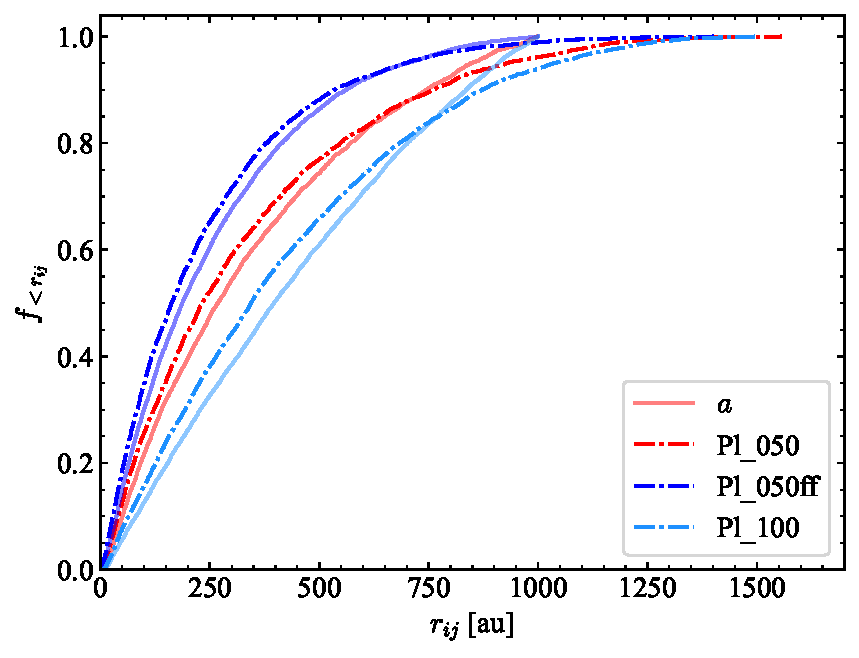
\includegraphics[width=\columnwidth]{figures/Plummer_General_proj_sep.pdf}
        \caption{CDF of surviving \jumbo\, projected separation distribution for models P05, P05FF, P1. Overplotted are translucent lines denoting the respective models' \jumbos\, semi-major axis.}
         \label{Fig:Plummer_rsep}
   \end{figure}
   \begin{figure}
    \centering
        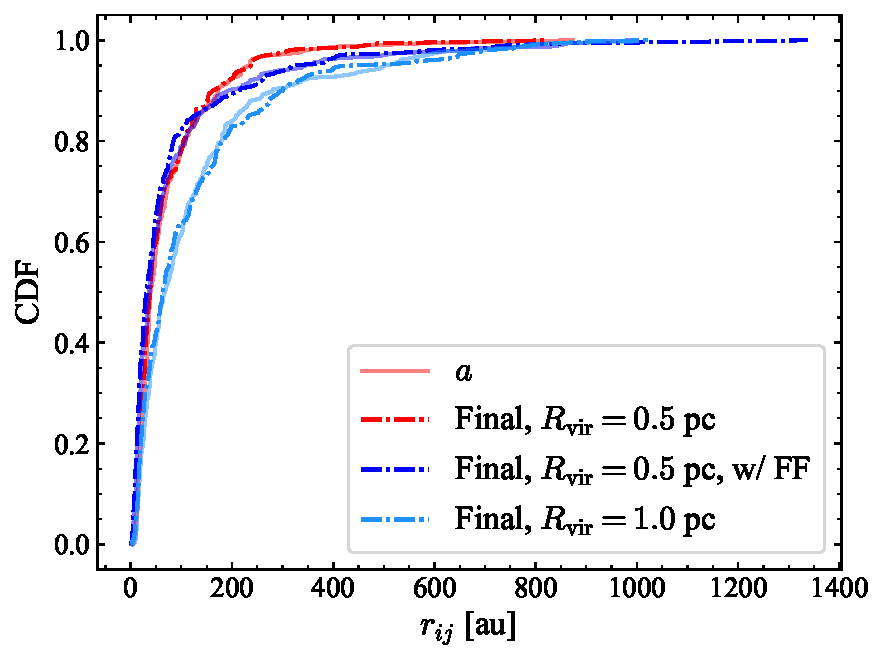
\includegraphics[width=\columnwidth]{figures/Fractal_General_proj_sep.pdf}
        \caption{CDF of surviving \jumbo\, projected separation distribution for models F05, F05FF, F1. Overplotted are translucent lines denoting the respective models' \jumbos\, semi-major axis.}
         \label{Fig:Fractal_rsep}
   \end{figure}
\end{appendix}


    
\end{document}

We conclude that the observed \jumbos\, in the Trapezium cluster
formed as planetary pairs together with the other stars.

\begin{table*}
 \caption{...}
 \label{Tab:model_ISF_vs_sma_rates}
 \centering 
 \begin{tabular}{lrrrrrrrrrrrr}
   \hline\hline
   model & $a_2$/au & $n_{(s,s)}$ & $n_{(s,p)}$ & $n_{p}$ & $n_{(p,p)}$ \\
        \hline \vspace{-0.75em}\\
%${\cal SPP}$\_Pl\_R025 &  0.0 & 197.6 & 1001 & 0.6 \\
${\cal ISF}$\_Fr\_R05 &  50 &  83.0 & 11.0 & 531.0 & 29.0 & 0 & 0 & 0 \\
${\cal ISF}$\_Fr\_R05 & 100 & 102.0 & 11.0 & 141.0 & 24.0 & 0 & 0 & 0 \\
${\cal ISF}$\_Fr\_R05 & 150 &  70.0 & 10.0 & 562.0 & 14.0 & 0 & 0 & 0 \\
${\cal ISF}$\_Fr\_R05 & 200 &  79.0 &  7.0 & 565.0 & 14.0 & 0 & 0 & 0 \\
${\cal ISF}$\_Fr\_R05 & 300 &  88.0 &  6.0 & 578.0 & 8.0 & 0 & 0 & 0 \\
${\cal ISF}$\_Fr\_R05 & 400 & 102.0 & 15.0 & 579.0 & 3.0 & 0 & 0 & 0 \\
${\cal ISF}$\_Fr\_R05 & 800 &  80.0 & 17.0 & 579.0 & 2.0 & 0 & 0 & 0 \\
${\cal ISF}$\_Fr\_R05 &1600 &  86.0 & 10.0 & 588.0 & 1.0 & 0 & 0 & 0 \\
\end{tabular}
\end{table*}

\begin{table*}
 \caption{...}
 \label{Tab:model_ISF_vs_sma_parameters}
 \centering 
 \begin{tabular}{lrrrrrrrrrrrr}
   \hline\hline
model &$a/au$ & $\langle M \rangle$ & $\langle m \rangle$ & $\langle a \rangle$ & $\langle e \rangle$ & $\langle d \rangle$ \\
        \hline \vspace{-0.75em}\\
%${\cal SPP}$\_Pl\_R025 &  0.0 & 197.6 & 1001 & 0.6 \\
${\cal ISF}$\_Fr\_R05 & 50 &$3.713^{+3.427}_{-1.494}$ & $0.731^{+0.405}_{-0.440}$ & $39.002^{+7.422}_{-5.958}$ & $0.502^{+0.228}_{-0.213}$& $33.830^{+12.064}_{-10.795}$  \\
${\cal ISF}$\_Fr\_R05 &100 &$6.032^{+2.538}_{-3.590}$ & $1.301^{+1.066}_{-0.679}$ & $47.183^{+17.561}_{-18.831}$ & $0.525^{+0.242}_{-0.225}$& $36.550^{+19.469}_{-16.452}$  \\
${\cal ISF}$\_Fr\_R05 &150 & $4.037^{+5.264}_{-1.552}$ & $0.638^{+1.067}_{-0.255}$ & $41.691^{+106.367}_{-9.897}$ & $0.700^{+0.166}_{-0.131}$& $53.255^{+40.398}_{-17.021}$  \\
${\cal ISF}$\_Fr\_R05 &200 &$4.223^{+1.716}_{-1.225}$ & $0.877^{+1.571}_{-0.463}$ & $43.394^{+23.126}_{-16.220}$ & $0.688^{+0.093}_{-0.336}$& $39.605^{+40.066}_{-17.487}$  \\
${\cal ISF}$\_Fr\_R05 &300 &$5.278^{+3.788}_{-2.439}$ & $1.291^{+1.537}_{-0.341}$ & $36.812^{+11.837}_{-7.330}$ & $0.573^{+0.239}_{-0.179}$& $46.200^{+7.743}_{-20.497}$  \\
${\cal ISF}$\_Fr\_R05 &400 &$3.332^{+6.031}_{-0.668}$ & $0.763^{+1.262}_{-0.285}$ & $37.815^{+62.038}_{-5.966}$ & $0.280^{+0.176}_{-0.077}$& $40.852^{+81.719}_{-4.104}$  \\
${\cal ISF}$\_Fr\_R05 &800 &$3.247^{+0.940}_{-0.940}$ & $0.388^{+0.080}_{-0.080}$ & $25.646^{+0.708}_{-0.708}$ & $0.480^{+0.019}_{-0.019}$& $20.344^{+10.236}_{-2.360}$  \\
${\cal ISF}$\_Fr\_R05 &1600 &$2.315^{+0.000}_{-0.000}$ & $0.056^{+0.000}_{-0.000}$ & $25.652^{+0.000}_{-0.000}$ & $0.116^{+0.000}_{-0.000}$& $20.912^{+1.166}_{-0.780}$  \\
\end{tabular}
\end{table*}




